\documentclass[a4paper, oneside, openany, dvipsnames, table]{article}
\usepackage{../../template/SWEightStyle}
\usepackage{ltablex}
\usepackage{tabularx}
\usepackage{pdfpages}
\usepackage{eurosym}
\usepackage{cleveref}
\usepackage{pdflscape}
\usepackage{float}


\setcounter{secnumdepth}{3}
\DeclareUnicodeCharacter{20AC}{\euro{}}
\newcommand{\Titolo}{Manuale Utente}

\newcommand{\Gruppo}{SWEight}

\newcommand{\Approvatore}{Damien Ciagola}
\newcommand{\Redattori}{Alberto Bacco \newline Sebastiano Caccaro \newline Gheorghe Isachi \newline Gionata Legrottaglie}
\newcommand{\Verificatori}{Francesco Corti \newline Francesco Magarotto}

\newcommand{\pathimg}{../template/img/logoSWEight.png}

\newcommand{\Versionedoc}{1.0.0}

\newcommand{\Distribuzione}{\proponente \newline Prof. Vardanega Tullio \newline Prof. Cardin Riccardo \newline Gruppo SWEight}

\newcommand{\Uso}{Esterno}

\newcommand{\NomeProgetto}{Colletta}

\newcommand{\Mail}{SWEightGroup@gmail.com}

\newcommand{\DescrizioneDoc}{Questo documento si occupa di fornire le modalità di utilizzo del software Colletta commissionato}


\begin{document}

\copertina{}

\definecolor{greySWEight}{RGB}{255, 71, 87}
\definecolor{greyROwSWEight}{RGB}{234, 234, 234}

\section*{Registro delle modifiche}
{
	\rowcolors{2}{greyROwSWEight}{white}
	\renewcommand{\arraystretch}{1.5}
	\centering
	\begin{longtable}{ c c C{4cm}  c  c }
		
		\rowcolor{greySWEight}
		\textcolor{white}{\textbf{Versione}} & \textcolor{white}{\textbf{Data}} & \textcolor{white}{\textbf{Descrizione}} & \textcolor{white}{\textbf{Nominativo}} & \textcolor{white}{\textbf{Ruolo}}\\
		1.2.2 & 2019-02-25 & Ampliamento sezione 5.4 e 3.2.5.2 & Alberto Bacco & \reda{} \\
		
		1.2.1 & 2019-02-23 & Aggiunta sezione 3.2.5.8 Checkstyle & Sebastiano Caccaro & \reda{} \\		
		
		1.2.0 & 2019-02-20 & Aggiunta scelte tecnologiche 3.2.4.2, da 3.4.5.4 a 3.4.5.7, 4.3.1.4, 4.3.2.2, 4.4.6 e figlie & Sebastiano Caccaro & \reda{} \\	
		
		1.1.5 & 2019-02-20 & Modifica sezione 2 & Alberto Bacco & \reda{} \\
		
		1.1.4 & 2019-02-18 & Correzione errori grammatica, spostate sottosezioni di asana da 4.3 a 5.2, & Alberto Bacco & \reda{} \\
		
		1.1.3 & 2019-02-14 & Riorganizzazione e correzione errori sezione 5 & Enrico Muraro & \reda{} \\
		
		1.1.2 & 2019-02-03 & Modifica sottosezione 4.1.10, 4.3.1.4, 4.3.1.5, 4.3.1.6 & Alberto Bacco& \reda{} \\	
		
		1.1.1 & 2019-01-31 & Modifica struttura e contenuti sezione 3  & Damien Ciagola & \reda{} \\	
		
		1.1.0 & 2019-01-27 & Sezione Qualità 4.2 & Sebastiano Caccaro & \reda{} \\	
		
		1.0.1 & 2019-01-25 & Parziale ristrutturazione della struttura del documento & Sebastiano Caccaro & \reda{} \\		
		
		1.0.0 & 2019-01-11 & Approvazione per il rilascio & Sebastiano Caccaro & \Res{} \\
		
		0.9.0 & 2019-01-9 & Verifica finale & Francesco Corti & \ver{} \\
		
		0.9.0 & 2019-01-8 & Aggiunta lista di controllo & Gionata Legrottaglie & \reda{} \\
		
		0.8.0 & 2018-12-23 & Correzioni errori ortografici & Gionata Legrottaglie & \reda{} \\
		
		0.7.0 & 2018-12-20 & Verifica documento & Francesco Corti & \ver{}\\
		
		0.6.0 & 2018-12-18 & Aggiunta sottosezione 5.2.2.2, 5.2.2.3, 5.2.2.4 & Francesco Magarotto & \reda{} \\
		
		0.5.2 & 2018-12-16 & Modifica sezione 4.1.5.3 & Alberto Bacco & \reda{} \\
		
		0.5.2 & 2018-12-16 & Modifica sezione 4.1.5.3 & Alberto Bacco & \reda{} \\
		
		0.5.2 & 2018-12-16 & Aggiunte sottosezioni  & Alberto Bacco & \reda{} \\
		
		0.5.1 & 2018-12-15 & Aggiunte sottosezioni 5.3, 5.4, 5.5, 5.6, 5.7, 5.8 & Alberto Bacco & \reda{} \\
		
		0.5.0 & 2018-12-15 & Aggiunta sezione 5 e sottosezioni 5.1, 5.2 & Gionata Legrottaglie & \reda{} \\
		
		0.4.1 & 2018-12-11 & Aggiunta sezione 4.1.7.3.1 & Francesco Magarotto & \reda{} \\ 
		
		0.4.0 & 2018-12-10 & Aggiunte sottosezioni 4.1.5, 4.1.6, 4.1.7, 4.1.8 & Gionata Legrottaglie & \reda{} \\ 
		0.4.0 & 2018-12-09 & Aggiunta sezione 4 e sottosezioni 4.1.1, 4.1.2, 4.1.3, 4.1.4 & Gionata Legrottaglie & \reda{} \\ 
		
		0.3.1 & 2018-12-07 & Aggiunta sottosezione 3.2 & Gionata Legrottaglie & \reda{} \\ 
		
		0.3.0 & 2018-12-06 & Aggiunta sezione 3 e sottosezione 3.1 & Gionata Legrottaglie & \reda{} \\ 
		
		0.2.0 & 2018-12-05 & Aggiunti i riferimenti & Gionata Legrottaglie & \reda{} \\ 
		
		0.1.0 & 2018-11-30 & Aggiunta introduzione & Gionata Legrottaglie & \reda{} \\
		
		0.0.1 & 2018-11-28 & Creazione scheletro del documento & Gionata Legrottaglie & \reda{}\\
		
	\end{longtable}

}
\newpage
\tableofcontents
\newpage
\listoffigures
\newpage
\listoftables
\newpage

\section{Introduzione}
	\subsection{Scopo del documento}
		% vecchia introduzione
% In questo documento è illustrata la {strategia}\ped{G} di {verifica}\ped{G} e 
% {validazione}\ped{G} del gruppo \gruppo . Tale strategia è fondamentale per dare una 
% misurazione oggettiva e quantificabile del livello di {qualità}\ped{G} di quanto viene 
% prodotto. \newline
% Ciò è vantaggioso sia per il gruppo \gruppo , che può facilmente individuare difetti 
% durante lo svolgimento del progetto, sia per il {committente}\ped{G}, che può costantemente 
% monitorare la qualità del prodotto in base a criteri oggettivi e prestabiliti.

% alternativa alla prima introduzione
In questo documento sono illustrate le {strategie}\ped{G} di {verifica}\ped{G}e 
{validazione}\ped{G} del gruppo \gruppo. 
Tale strategia ci si assicura la qualità dei processi, dei documenti e delle procedure 
utilizzate per gestire e sviluppare i risultati finali.
Lo scopo di questo documento è descrivere le informazioni necessarie per gestire efficacemente 
la qualità del progetto, dalla pianificazione alla consegna, comprendendo obiettivi 
di qualità, responsabilità, e l'approccio di gestione della qualità per 
garantire che gli obiettivi siano raggiunti.\newline
Ciò è vantaggioso sia per il gruppo \gruppo , che può facilmente individuare difetti 
durante lo svolgimento del progetto, sia per il {committente}\ped{G}, che può costantemente 
monitorare la qualità del prodotto in base a criteri oggettivi e prestabiliti.


	\subsection{Scopo del prodotto}
		Il progetto prevede la realizzazione di una piattaforma collaborativa di raccolta dati in cui gli utenti possano predisporre e/o svolgere piccoli esercizi di analisi grammaticale. Lo scopo è raccogliere dati relativi sia  agli esercizi predisposti, che al loro svolgimento da parte degli utenti. Sviluppatori e ricercatori utilizzeranno queste informazione per insegnare ad un elaboratore a svolgere i medesimi esercizi, mediante tecniche di apprendimento automatico.

%Questa parte è un copia-incolla cafonissimo dal capitolato della mivoc
%Siccome è proprio quello che vogliono, non mi sembrava il caso di andare a modifcarla
	\subsection{Glossario}
		
\section*{F}
\textbf{Freeling}: the library for pos-tagging developed by TALP Research Center written in C++;
\section*{P}
\textbf{Pos-tagging}: part-of-speech tagging, also called grammatical tagging or word-category disambiguation, is the process of marking up a word in a text (corpus) as corresponding to a particular part of speech; \\ 
\textbf{POJO}: Plain Old Java Object, is an ordinary Java object, not bound by any special restriction and not requiring any class path. In Spring it refers to a Java object (instance of definition) that isn't bogged down by framework extensions;
\section*{J}
\textbf{JSON}: JavaScript Object Notation, is a lightweight data-interchange format.  It is easy for humans to read and write. It is easy for machines to parse and generate.\\
\textbf{JWT}: JSON Web Token, a JSON-based open standard (RFC 7519) for creating access tokens that assert some number of claims;

	\subsection{Riferimenti}
		\subsubsection{Riferimenti normativi}
			\begin{itemize}
	\item \textbf{Norme di Progetto:} \NdP ;
	\item \textbf{Capitolato d'appalto C2: } Colletta \newline
		  \url{https://www.math.unipd.it/~tullio/IS-1/2018/Progetto/C2.pdf}.
\end{itemize}
		\subsubsection{Riferimenti informativi}
		\label{sec:RifInf}
			\begin{itemize}
    \item Software Engineering (10th edition) - Ian Sommerville
    \item Slide "Gestione di Progetto", corso di Ingegneria del Software
          \newline \url{https://www.math.unipd.it/~tullio/IS-1/2018/Dispense/L06.pdf}
\end{itemize}
	\subsection{Scadenze}
		Il gruppo \gruppo\space si imppegna a rispettare le seguenti scadenze, sulle quali
è basata la pianficazione del progetto.

\rowcolors{2}{greyROwSWEight}{white}
\renewcommand{\arraystretch}{1.5}
\begin{table}[H]	
	\begin{center}
	    \begin{tabular}{| c | c | }
	        \hline
	        \rowcolor{greySWEight}
	        \textcolor{white}{\textbf{Revisione}} & \textcolor{white}{\textbf{Scadenza}}\\
	        RR & 21/01/2019 \\
	        RP & 15/03/2019 \\
	        RQ & 19/04/2019 \\
	        RA & 17/05/2019 \\
	        \hline
	    \end{tabular}
	    \caption{Scadenze} \label{tab:tabellascadenze} 
	\end{center}
\end{table}

   
\newpage
\section{Analisi dei rischi}
	\label{sec:rischi}
	\subsection{Document goal}
The purpose of this document is to provide all the necessary information to extend, correct and improve Colletta.
There will be additional information regarding setting up the development environment to work in an environment that is as consistent as possible with that used
by the other members of group SWEight, but can be ignored if you only want to use part of the product.
This guide was written taking into account the Microsoft Windows and Linux operating systems. If other systems are used, compatibility issues may arise, even if it's unlikely. In this case refer to the git page. This document will grow as the product will be fully
developed.

\subsection{Product goal}
The purpose of the product is the creation of a collaborative data collection platform where users can prepare and/or perform small grammar exercises. 
The front-end of the system consists of a web application developed with React and Redux, while the back-end is a Spring Boot application written in Java, which will handle HTTP Requests sent from the front-end. 

\subsection{References}


\subsubsection{Installation references}

\begin{itemize}
\item \textbf{Git}: \url{https://git-scm.com/}
\item \textbf{Node.js}: \url{https://nodejs.org/en/}
\item \textbf{NPM}: \url{https://www.npmjs.com/}
\item \textbf{Oracle JDK}: \url{https://www.oracle.com/technetwork/java/javase/downloads/index.html}
\item \textbf{OpenJDK}: \url{https://openjdk.java.net/}
\item \textbf{Maven}: \url{https://maven.apache.org/}
\item \textbf{Lombok}: \url{https://projectlombok.org/}
\item \textbf{VSCode}: \url{https://code.visualstudio.com/} 

\end{itemize}

\subsubsection{Legal references}
\begin{itemize}
\item \textbf{MIT License}: \url{https://opensource.org/licenses/MIT}
\end{itemize}

%\subsubsection{Informative references}

	\newpage
	\newcommand{\barra}{\hline \hline \hline}
\renewcommand{\arraystretch}{1.5}
\def\tabularxcolumn#1{m{#1}}
\begin{tabularx}{\textwidth}{C{0.2\textwidth} X C{0.2\textwidth}}
\hline
\rowcolor{greySWEight}
    \textcolor{white}{\textbf{Nome}} & \textcolor{white}{\textbf{Descrizione}}&
    \textcolor{white}{\textbf{Livello di Rischio}}\endhead
\hline
 \textbf  	
 	{Conflitti fra i membri del gruppo}&
    Per molti membri del gruppo questa è la prima esperienza di lavoro in gruppo con un certo
    numero di persone.Ciò potrebbe causare inconvenienti di natura interpersonale.&
    
    Probabilità: \newline \textbf{Bassa}\newline
    Gravità: \newline \textbf{Alta}\\
    
    Contromisure &
    \multicolumn{2}{L{\dimexpr\textwidth-4\tabcolsep-0.2\textwidth}}{
    Ogni problema andrà tempestivamente riportato al responsabile. Ove non sia possibile
    trovare una soluzione, il responsabile cercherà di assegnare ruoli e attività che 
    minimizzino l'interazione fra i membri in causa.
    }\\
    \barra
    
    
 
 \textbf
 	{Assenza prolungata di un membro del gruppo}&
    \'E possibile che, a causa di problemi di salute o familiari, un membro del gruppo possa
    non poter svolgere le sue mansioni per un certo periodo di tempo. &
    Probabilità: \newline \textbf{Bassa}\newline
    Gravità: \newline \textbf{Alta}\\
    
    Contromisure&
    \multicolumn{2}{L{\dimexpr\textwidth-4\tabcolsep-0.2\textwidth}}{
    A seconda della natura del problema e delle attività lasciate in sospeso, il responsabile
    può ridistribuire il carico di lavoro del membro assente o posticiparle e rivedere
    la pianificazione
    }\\
    \barra

\textbf
    {Incompatibilità orari dei membri del gruppo}&
   A causa di ubicazione geografica e diversi impegni universitari e lavorativi
   dei vari membri del gruppo, può essere complicato incontrarsi di persona per
   discutere del progetto.&
   Probabilità: \newline \textbf{Alta}\newline
   Gravità: \newline \textbf{Bassa}\\
   
   Contromisure&
   \multicolumn{2}{L{\dimexpr\textwidth-4\tabcolsep-0.2\textwidth}}{
   Creazione di una tabella oraria con gli impegni di ogni membro del gruppo. \newline
   Ogni riunione avrà uno scopo ben preciso, e ogni membro è tenuto a preparasi
   attentamente per sfruttare al meglio il tempo disponibile. \newline
   In caso non sia possibile organizzare un incontro fisico, è sempre possibile
   discutere in videoconferenza.
   Una riunione può essere svolta anche in assenza 2 membri.
   }\\
   \barra
   
\textbf
    {Incompatibilità orari dei membri del gruppo}&
   A causa di ubicazione geografica e diversi impegni universitari e lavorativi
   dei vari membri del gruppo, può essere complicato incontrarsi di persona per
   discutere del progetto.&
   Probabilità: \newline \textbf{Alta}\newline
   Gravità: \newline \textbf{Bassa}\\
   
   Contromisure&
   \multicolumn{2}{L{\dimexpr\textwidth-4\tabcolsep-0.2\textwidth}}{    
   Creazione di una tabella oraria con gli impegni di ogni membro del gruppo. \newline
   Ogni riunione avrà uno scopo ben preciso, e ogni membro è tenuto a preparasi
   attentamente per sfruttare al meglio il tempo disponibile. \newline
   In caso non sia possibile organizzare un incontro fisico, è sempre possibile
   discutere in videoconferenza.
   Una riunione può essere svolta anche in assenza 2 membri.
   }\\
   \barra
   
\textbf
    {Inesperienza tecnologica}&
   Alcuni membri del gruppo potrebbero non conoscere alcune delle tecnologie utilizzate nel
   progetto&
   Probabilità: \newline \textbf{Alta}\newline
   Gravità: \newline \textbf{Media}\\
   
   Contromisure&
   \multicolumn{2}{L{\dimexpr\textwidth-4\tabcolsep-0.2\textwidth}}{    
   Studio individuale delle tecnologie sconosciute, eventualmente coadiuvato da un membro più
   esperto in una determinata tecnologia. L'assegnazione delle attività deve tenere conto delle
   conoscenze tecnologiche degli assegnatari.
   }\\
   \barra
   
   	{Danni hardware e software}&
   Possibili malfunzionamenti agli strumenti di lavoro possono rallentare lo svolgimento delle attività o
   causare la perdita di lavoro già svolto.
   &
   Probabilità: \newline \textbf{Bassa}\newline
   Gravità: \newline \textbf{Media}\\
   
   Contromisure&
   \multicolumn{2}{L{\dimexpr\textwidth-4\tabcolsep-0.2\textwidth}}{    
   Ogni incremento significativo nello svolgimento di un'attività va tempestivamente versionato nel cloud.
 
   }\\
   \barra

   {Inesperienza organizzativa}&
   Nessuno dei membri del team ha mai lavorato ad un progetto con questo livello di organizzazione.
   Pertanto, può risultare difficile stimare il costo temporale delle attività e organizzare quest'ultime
   nel tempo.
   &
   Probabilità: \newline \textbf{Alta}\newline
   Gravità: \newline \textbf{Media}\\
   
   Contromisure&
   \multicolumn{2}{L{\dimexpr\textwidth-4\tabcolsep-0.2\textwidth}}{    
   Ogni attività è comprensiva di un periodo di slack. Pianificare milestone più frequenti durante le prime
   fasi del progetto, in modo da limitare il margine di errore e da correggere il tiro con i consuntivi.
 
   }\\
   \barra
\caption{Analisi dei rischi} \label{tab:sometab} 
\end{tabularx}




\newpage
\section{Modelli di sviluppo}
	\subsection{Document goal}
The purpose of this document is to provide all the necessary information to extend, correct and improve Colletta.
There will be additional information regarding setting up the development environment to work in an environment that is as consistent as possible with that used
by the other members of group SWEight, but can be ignored if you only want to use part of the product.
This guide was written taking into account the Microsoft Windows and Linux operating systems. If other systems are used, compatibility issues may arise, even if it's unlikely. In this case refer to the git page. This document will grow as the product will be fully
developed.

\subsection{Product goal}
The purpose of the product is the creation of a collaborative data collection platform where users can prepare and/or perform small grammar exercises. 
The front-end of the system consists of a web application developed with React and Redux, while the back-end is a Spring Boot application written in Java, which will handle HTTP Requests sent from the front-end. 

\subsection{References}


\subsubsection{Installation references}

\begin{itemize}
\item \textbf{Git}: \url{https://git-scm.com/}
\item \textbf{Node.js}: \url{https://nodejs.org/en/}
\item \textbf{NPM}: \url{https://www.npmjs.com/}
\item \textbf{Oracle JDK}: \url{https://www.oracle.com/technetwork/java/javase/downloads/index.html}
\item \textbf{OpenJDK}: \url{https://openjdk.java.net/}
\item \textbf{Maven}: \url{https://maven.apache.org/}
\item \textbf{Lombok}: \url{https://projectlombok.org/}
\item \textbf{VSCode}: \url{https://code.visualstudio.com/} 

\end{itemize}

\subsubsection{Legal references}
\begin{itemize}
\item \textbf{MIT License}: \url{https://opensource.org/licenses/MIT}
\end{itemize}

%\subsubsection{Informative references}

	\subsection{Ciclo di vita del software}
		L'analisi dei rischi ha stimato un basso rischio di cambio dei requisiti da parte della proponente.
Ciò significa che è possibile adottare un modello di sviluppo che prevede un'approfondita fase di 
analisi e progettazione iniziale.
La scelta è quindi ricaduta sul modello di sviluppo incrementale, che, inoltre, presenta altre
caratteristiche congeniali alle intenzioni del gruppo \gruppo \space :
\begin{itemize}
    \item Lo sviluppo del prodotto software è diviso in varie attività singole, comportando i seguenti vantaggi:
    \begin{itemize}
    	\item Maggior semplicità dello sviluppo di un'attività
    	\item Maggior semplicità in fase di test e troubleshooting
    	\item Migliore parallelizzazione del lavoro
    	\item Minore probabilità di incorrere in ritardi
    	\item Maggiore facilità nel rilascio
    \end{itemize}
    \item Le suddette attività sono ordinate in ordine di importanza, e vengono sviluppati prima i requisti di maggiore rilevanza per il committente
    \item Creazione di milestone per suddividere meglio il lavoro e per ottenere riscontri dal committente sul soddisfacimento dei requisiti
\end{itemize}
\newpage
\section{Pianificazione}
	\label{sec:Pian}
	\subsection{Document goal}
The purpose of this document is to provide all the necessary information to extend, correct and improve Colletta.
There will be additional information regarding setting up the development environment to work in an environment that is as consistent as possible with that used
by the other members of group SWEight, but can be ignored if you only want to use part of the product.
This guide was written taking into account the Microsoft Windows and Linux operating systems. If other systems are used, compatibility issues may arise, even if it's unlikely. In this case refer to the git page. This document will grow as the product will be fully
developed.

\subsection{Product goal}
The purpose of the product is the creation of a collaborative data collection platform where users can prepare and/or perform small grammar exercises. 
The front-end of the system consists of a web application developed with React and Redux, while the back-end is a Spring Boot application written in Java, which will handle HTTP Requests sent from the front-end. 

\subsection{References}


\subsubsection{Installation references}

\begin{itemize}
\item \textbf{Git}: \url{https://git-scm.com/}
\item \textbf{Node.js}: \url{https://nodejs.org/en/}
\item \textbf{NPM}: \url{https://www.npmjs.com/}
\item \textbf{Oracle JDK}: \url{https://www.oracle.com/technetwork/java/javase/downloads/index.html}
\item \textbf{OpenJDK}: \url{https://openjdk.java.net/}
\item \textbf{Maven}: \url{https://maven.apache.org/}
\item \textbf{Lombok}: \url{https://projectlombok.org/}
\item \textbf{VSCode}: \url{https://code.visualstudio.com/} 

\end{itemize}

\subsubsection{Legal references}
\begin{itemize}
\item \textbf{MIT License}: \url{https://opensource.org/licenses/MIT}
\end{itemize}

%\subsubsection{Informative references}

	\newpage	
	\subsection{Analisi}
		Nella seguente tabella è illustrato il consuntivo del periodo di Analisi.

\begin{table}[H]
\centering
\begin{tabular}{c|ccc|ccc}
\rowcolor{greySWEight}
\multicolumn{1}{c}{} & \multicolumn{3}{c}{\textcolor{white}{\textbf{Ore}}} & \multicolumn{3}{c}{\textcolor{white}{\textbf{Costo in Euro}}} \\
{\textbf{Ruolo}} & {\textbf{Preventivo}} & {\textbf{Consuntivo}} & {\textbf{Delta}} & {\textbf{Preventivo}} & {\textbf{Consuntivo}} & {\textbf{Delta}} \\
Responsabile & 20 & 24 & +4 &  600,00 &  720,00 & + 120,00 \\
Amministratore & 20 & 22 & +2 &  400,00 &  440,00 & + 40,00 \\
Analista & 70 & 74 & +4 &  1.750,00 &  1.850,00 & + 100,00 \\
Progettista & 0 & 0 & 0 &  0,00 &  0,00 &  0,00 \\
Programmatore & 0 & 0 & 0 &  0,00 &  0,00 &  0,00 \\
Verificatore & 50 & 46 & -4 &  750,00 &  690,00 & - 60,00 \\
\hline
\textbf{Totale} & \textbf{160} & \textbf{166} & \textbf{+6} &  \textbf{3.500,00} &  \textbf{3.700,00} & \textbf{+ 200,00} \\


\end{tabular}
\caption{Consuntivo del periodo di Analisi}
\end{table}

	\newpage	
	\subsection{Consolidamento}
		\subsubsection{Prospetto Orario}
Di seguito è riportata la suddivisione oraria dei ruoli nel periodo di Consolidamento.




\begin{table}[H]	
	\begin{center}
	    \begin{tabular}{cccccccc}
	  		
			\rowcolor{greySWEight}
			\textcolor{white}{\textbf{Nome}} & \textcolor{white}{\textbf{Re}} & \textcolor{white}{\textbf{Am}} & \textcolor{white}{\textbf{An}} & \textcolor{white}{\textbf{Pj}} & \textcolor{white}{\textbf{Pr}} & \textcolor{white}{\textbf{Ve}} & \textcolor{white}{\textbf{Totale}}
			\\ \hline
			Bacco Alberto & 5 & & & & & & 5 \\
			Caccaro Sebastiano & & & & & & 5 & 5 \\
			Ciagola Damien & & 5 & & & & & 5 \\
			Corti Francesco & & & & & & 5 & 5 \\
			Isachi Gheorghe & & 5 & & & & & 5 \\
			Legrottagle Gionata & & & 5 & & & & 5 \\
			Magarotto Francesco & & & & & & 5 & 5 \\
			Muraro Enrico & & & & & & 5 & 5 \\

			\end{tabular}
	    \caption{Tabella della suddivisione oraria dei membri del gruppo nel periodo di Consolidamento} \label{tab:tabellaPersoneConsolidamento} 
	\end{center}
\end{table}

La tabella della suddivisione oraria è rappresentata nel seguente grafico.
\begin{figure}[H]
	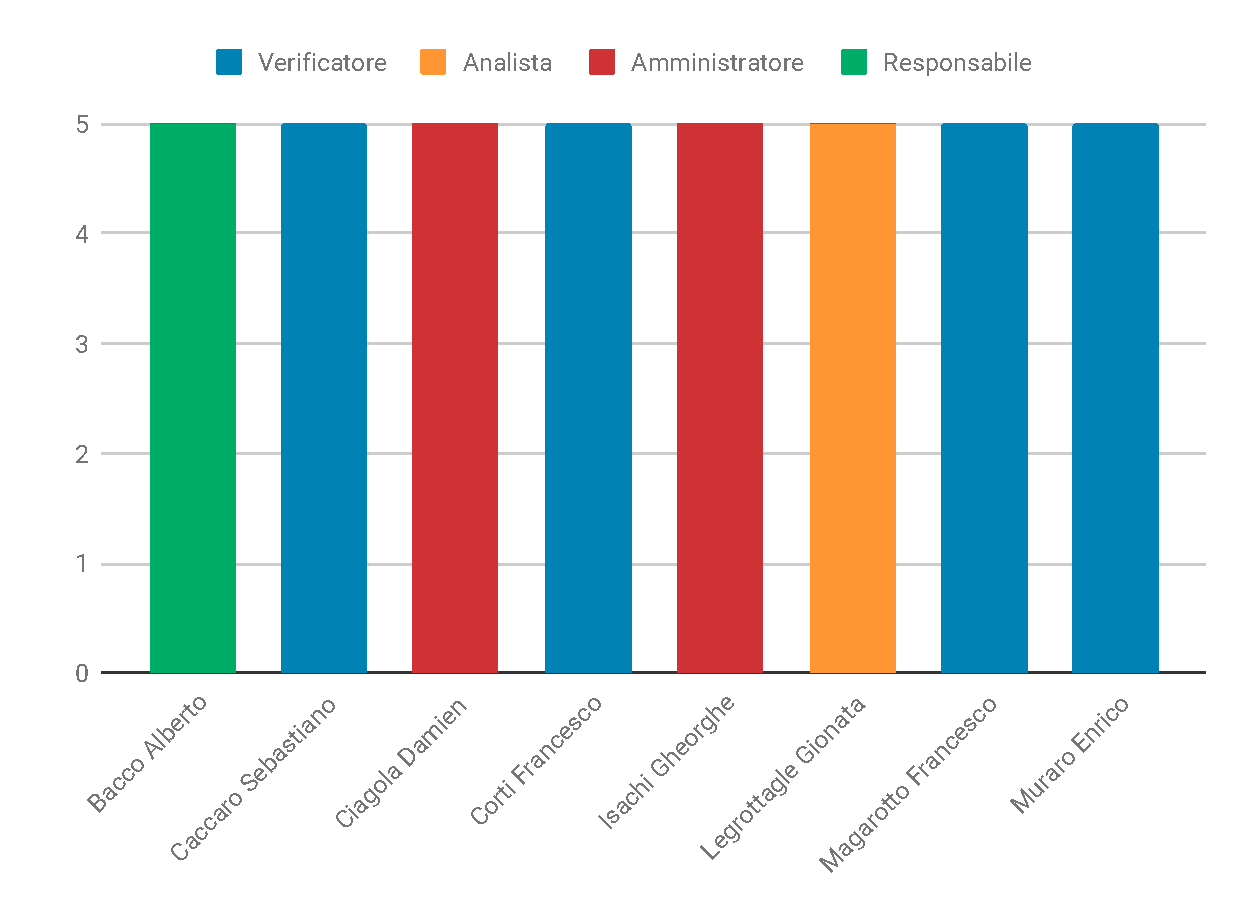
\includegraphics[width=1\linewidth]{Preventivo/grafici/CO1.pdf}
	\caption{Grafico della suddivisione oraria dei membri del gruppo nel periodo di Consolidamento}
\end{figure}

\subsubsection{Prospetto Economico}
Nella seguente tabella sono riportate le ore e i costi preventivati per ogni ruolo durante la fase di Consolidamento.


\begin{table}[H]	
	\begin{center}
	    \begin{tabular}{C{4cm}C{1cm}C{3,5cm}}
			\rowcolor{greySWEight}
			\textcolor{white}{\textbf{Ruolo}} & \textcolor{white}{\textbf{Ore}} & \textcolor{white}{\textbf{Costo}}
			\\ \hline
			Responsabile & 5 & \euro \space 150,00 \\
			Amministratore & 10 & \euro \space 200,00 \\
			Analista & 5 & \euro \space 125,00 \\
			Progettista &  & \\
			Programmatore &  &  \\
			Verificatore & 20 & \euro \space 300,00 \\
			\textbf{Totale} & \textbf{40} & \euro \space \textbf{775,00} \\
		\end{tabular}
	    \caption{Tabella della suddivisione oraria dei ruoli nel periodo di Consolidamento} \label{tab:tabellaRuoliConsolidamento} 
	\end{center}
\end{table}


Si può avere una più chiara rappresentazione della distribuzione oraria dei ruoli nel seguente grafico.

\begin{figure}[H]
	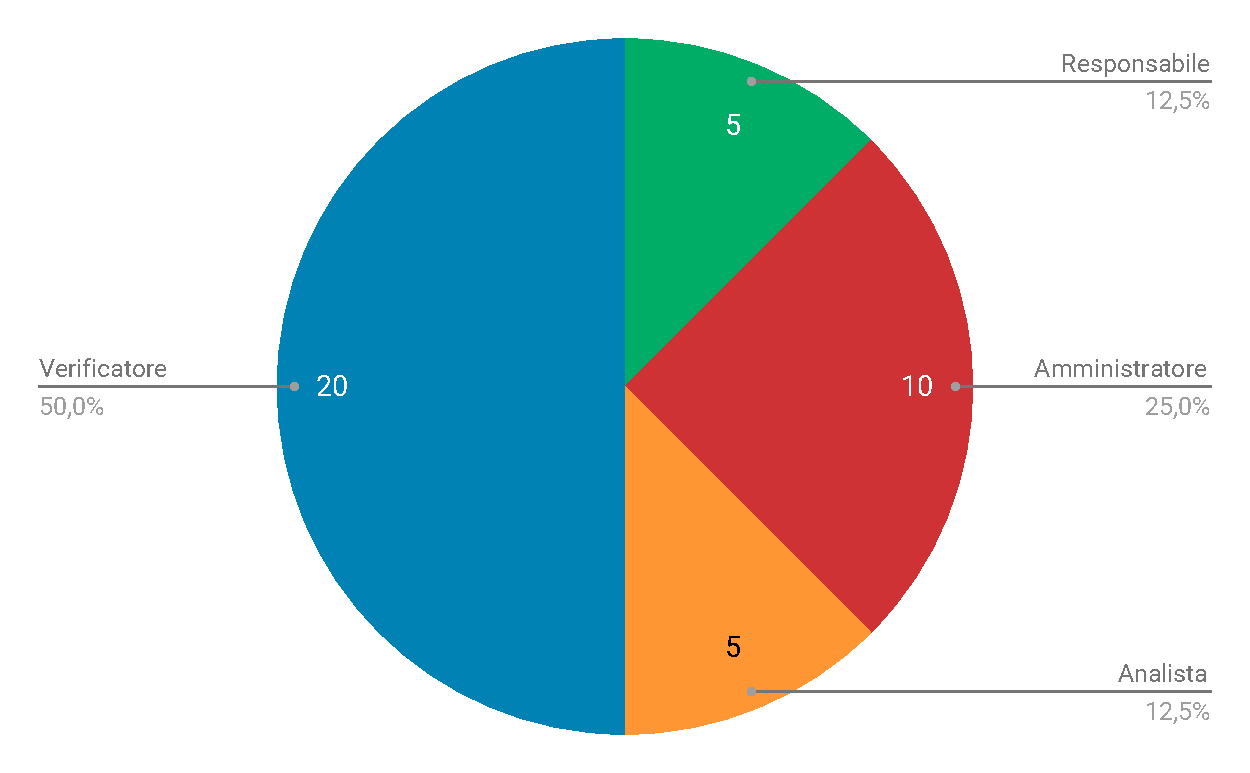
\includegraphics[width=1\linewidth]{Preventivo/grafici/CO2.pdf}
	\caption{Grafico della suddivisione oraria dei ruoli nel periodo di Consolidamento}
\end{figure}


	\newpage
	\subsection{Progettazione Architetturale}
		\subsubsection{Prospetto Orario}
Di seguito è riportata la suddivisione oraria dei ruoli nel periodo di Progettazione Architetturale.




\begin{table}[H]	
	\begin{center}
	    \begin{tabular}{cccccccc}
			\rowcolor{greySWEight}
			\textcolor{white}{\textbf{Nome}} & \textcolor{white}{\textbf{Re}} & \textcolor{white}{\textbf{Am}} & \textcolor{white}{\textbf{An}} & \textcolor{white}{\textbf{Pj}} & \textcolor{white}{\textbf{Pr}} & \textcolor{white}{\textbf{Ve}} & \textcolor{white}{\textbf{Totale}}
			\\
			Bacco Alberto & 5 & & 7 & 5 & & 12 & 29 \\
			Caccaro Sebastiano & & & & 12 & & 17 & 29 \\
			Ciagola Damien & & & & 12 & & 17 & 29 \\
			Corti Francesco & & 5 & & 15 & & 9 & 29 \\
			Isachi Gheorghe & & & & 14 & & 15 & 29 \\
			Legrottagle Gionata & & & & 27 & & 2 & 29 \\
			Magarotto Francesco & 5 & & & 24 & & & 29 \\
			Muraro Enrico & & 5 & & 24 & & & 29 \\
			\end{tabular}
	    \caption{Tabella della suddivisione oraria dei membri del gruppo nel periodo di Progettazione Architetturale} \label{tab:tabellaPersoneProgettazione Architetturale} 
	\end{center}
\end{table}

La tabella della suddivisione oraria è rappresentata nel seguente grafico.
\begin{figure}[H]
	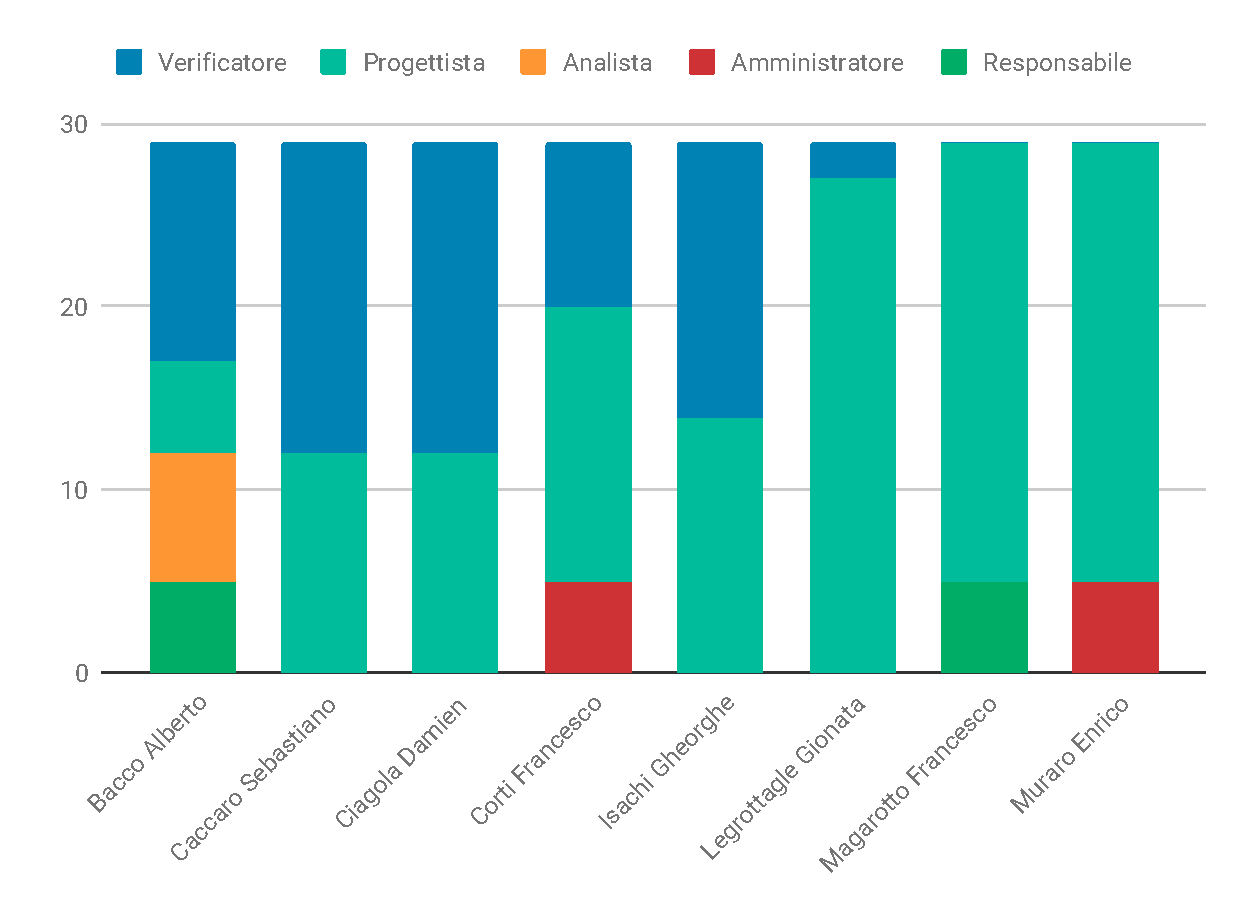
\includegraphics[width=1\linewidth]{Preventivo/grafici/PA1.pdf}
	\caption{Grafico della suddivisione oraria dei membri del gruppo nel periodo di Progettazione Architetturale}
\end{figure}

\subsubsection{Prospetto Economico}
Nella seguente tabella sono riportate le ore e i costi preventivati per ogni ruolo durante la fase di Progettazione Architetturale.


\begin{table}[H]	
	\begin{center}
	    \begin{tabular}{C{4cm}C{1cm}C{3,5cm}}
			\rowcolor{greySWEight}
			\textcolor{white}{\textbf{Ruolo}} & \textcolor{white}{\textbf{Ore}} & \textcolor{white}{\textbf{Costo}}
			\\
			Responsabile & 10 & \euro \space  300,00 \\
			Amministratore & 10 & \euro \space  200,00 \\
			Analista & 7 & \euro \space  175,00 \\
			Progettista & 133 & \euro \space  2.926,00 \\
			Programmatore &  & \euro \space  \\
			Verificatore & 72 & \euro \space  1.080,00 \\
			\textbf{Totale} & \textbf{232} & \euro \space  \textbf{4.681,00} \\
		\end{tabular}
	    \caption{Tabella della suddivisione oraria dei ruoli nel periodo di Progettazione Architetturale} \label{tab:tabellaRuoliProgettazione Architetturale} 
	\end{center}
\end{table}


Si può avere una più chiara rappresentazione della distribuzione oraria dei ruoli nel seguente grafico.

\begin{figure}[H]
	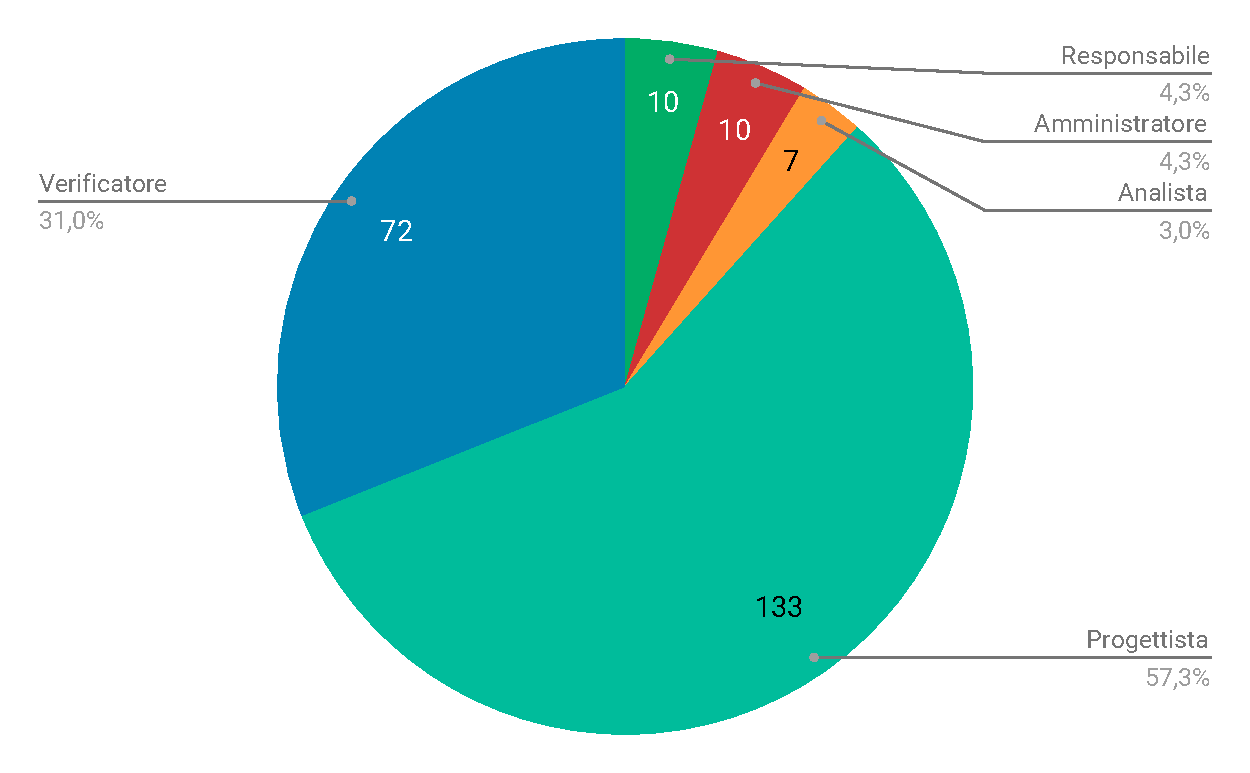
\includegraphics[width=1\linewidth]{Preventivo/grafici/PA2.pdf}
	\caption{Grafico della suddivisione oraria dei ruoli nel periodo di Progettazione Architetturale}
\end{figure}


	\newpage
	\subsection{Pianificazione di Dettaglio e Codifica}
		Il periodo di Progettazione di dettaglio e codifica inizia con la consegna della RP e termina con la consegna della RQ.\newline
Durante questo periodo, vengono svolte le seguenti attività:
\begin{itemize}
	\item \textbf{Incremento: }modifiche incrementali ai seguenti documenti, ove necessario:
	\begin{itemize}
		\item Analisi dei requisiti;
		\item Piano di progetto;
		\item Piano di qualifica;
		\item Glossario;
		\item Norme di progetto;
		\item Specifica Tecnica;
	\end{itemize}
	\item \textbf{Product Baseline: }sulla base della specifica tecnica viene redatto il documento di definizione di prodotto, nella quale sono contenute le scelte progettuali di dettaglio;
	\item \textbf{Codifica: }basandosi sulla definizione di prodotto, viene scritto il codice sorgente;
	\item \textbf{Manuale Utente: }redazione del manuale utente del prodotto. 
\end{itemize}


\begin{figure}[H]
	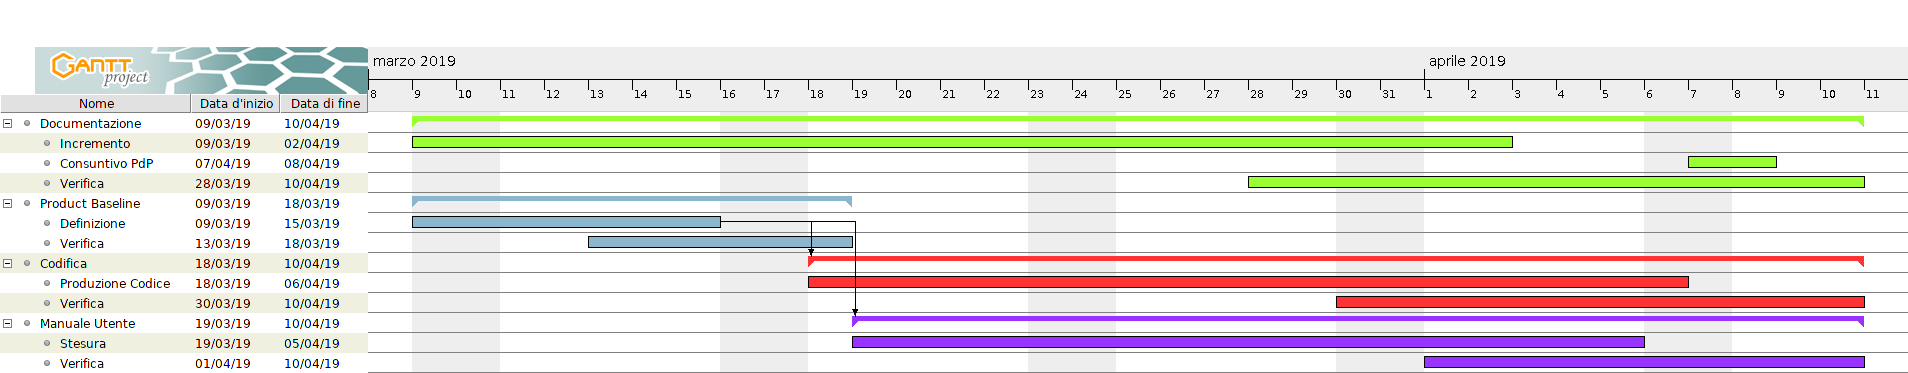
\includegraphics[width=1\linewidth]{Pianificazione/Progettazione_Dettaglio_Codififca.png}
	\caption{Diagramma di Gantt del periodo di Progettazione di dettaglio e codifica}
\end{figure}
	\newpage
	\subsection{Verifica e Validazione}
		Il periodo di verifica e validazione inizia con la consegna della RQ e termina con la consegna della RA.\newline
Durante questo periodo, sono svolte le seguenti attività:
\begin{itemize}
	\item \textbf{Incremento: }modifiche incrementali ai seguenti documenti, ove necessario:
	\begin{itemize}
		\item Analisi dei requisiti;
		\item Piano di progetto;
		\item Piano di qualifica;
		\item Glossario;
		\item Norme di progetto;
		\item Specifica Tecnica;
		\item Definizione di Prodotto;
		\item Manuale Utente;
	\end{itemize}
	\item \textbf{Validazione e collaudo: }il prodotto viene testato per accertarsi che soddisfi tutti i requisiti prestabiliti.
\end{itemize}


\begin{figure}[H]
	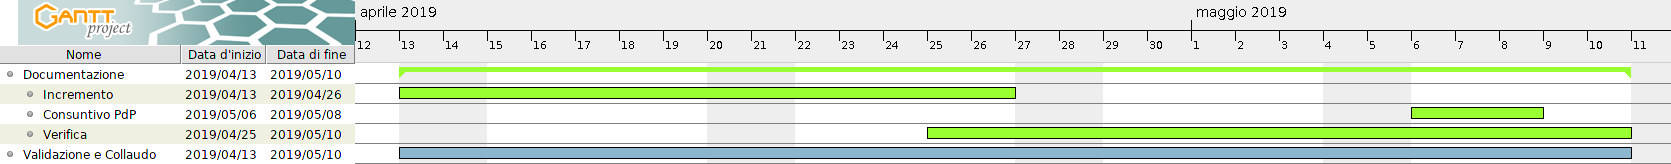
\includegraphics[width=1\linewidth]{Pianificazione/Verifica_Validazione.png}
	\caption{Diagramma di Gantt del periodo di verifica e validazione}
\end{figure}
\newpage
\section{Preventivo}
	\subsection{Document goal}
The purpose of this document is to provide all the necessary information to extend, correct and improve Colletta.
There will be additional information regarding setting up the development environment to work in an environment that is as consistent as possible with that used
by the other members of group SWEight, but can be ignored if you only want to use part of the product.
This guide was written taking into account the Microsoft Windows and Linux operating systems. If other systems are used, compatibility issues may arise, even if it's unlikely. In this case refer to the git page. This document will grow as the product will be fully
developed.

\subsection{Product goal}
The purpose of the product is the creation of a collaborative data collection platform where users can prepare and/or perform small grammar exercises. 
The front-end of the system consists of a web application developed with React and Redux, while the back-end is a Spring Boot application written in Java, which will handle HTTP Requests sent from the front-end. 

\subsection{References}


\subsubsection{Installation references}

\begin{itemize}
\item \textbf{Git}: \url{https://git-scm.com/}
\item \textbf{Node.js}: \url{https://nodejs.org/en/}
\item \textbf{NPM}: \url{https://www.npmjs.com/}
\item \textbf{Oracle JDK}: \url{https://www.oracle.com/technetwork/java/javase/downloads/index.html}
\item \textbf{OpenJDK}: \url{https://openjdk.java.net/}
\item \textbf{Maven}: \url{https://maven.apache.org/}
\item \textbf{Lombok}: \url{https://projectlombok.org/}
\item \textbf{VSCode}: \url{https://code.visualstudio.com/} 

\end{itemize}

\subsubsection{Legal references}
\begin{itemize}
\item \textbf{MIT License}: \url{https://opensource.org/licenses/MIT}
\end{itemize}

%\subsubsection{Informative references}

	\newpage
	\subsection{Analisi}
	    Nella seguente tabella è illustrato il consuntivo del periodo di Analisi.

\begin{table}[H]
\centering
\begin{tabular}{c|ccc|ccc}
\rowcolor{greySWEight}
\multicolumn{1}{c}{} & \multicolumn{3}{c}{\textcolor{white}{\textbf{Ore}}} & \multicolumn{3}{c}{\textcolor{white}{\textbf{Costo in Euro}}} \\
{\textbf{Ruolo}} & {\textbf{Preventivo}} & {\textbf{Consuntivo}} & {\textbf{Delta}} & {\textbf{Preventivo}} & {\textbf{Consuntivo}} & {\textbf{Delta}} \\
Responsabile & 20 & 24 & +4 &  600,00 &  720,00 & + 120,00 \\
Amministratore & 20 & 22 & +2 &  400,00 &  440,00 & + 40,00 \\
Analista & 70 & 74 & +4 &  1.750,00 &  1.850,00 & + 100,00 \\
Progettista & 0 & 0 & 0 &  0,00 &  0,00 &  0,00 \\
Programmatore & 0 & 0 & 0 &  0,00 &  0,00 &  0,00 \\
Verificatore & 50 & 46 & -4 &  750,00 &  690,00 & - 60,00 \\
\hline
\textbf{Totale} & \textbf{160} & \textbf{166} & \textbf{+6} &  \textbf{3.500,00} &  \textbf{3.700,00} & \textbf{+ 200,00} \\


\end{tabular}
\caption{Consuntivo del periodo di Analisi}
\end{table}

	\newpage	
	\subsection{Consolidamento}
	    \subsubsection{Prospetto Orario}
Di seguito è riportata la suddivisione oraria dei ruoli nel periodo di Consolidamento.




\begin{table}[H]	
	\begin{center}
	    \begin{tabular}{cccccccc}
	  		
			\rowcolor{greySWEight}
			\textcolor{white}{\textbf{Nome}} & \textcolor{white}{\textbf{Re}} & \textcolor{white}{\textbf{Am}} & \textcolor{white}{\textbf{An}} & \textcolor{white}{\textbf{Pj}} & \textcolor{white}{\textbf{Pr}} & \textcolor{white}{\textbf{Ve}} & \textcolor{white}{\textbf{Totale}}
			\\ \hline
			Bacco Alberto & 5 & & & & & & 5 \\
			Caccaro Sebastiano & & & & & & 5 & 5 \\
			Ciagola Damien & & 5 & & & & & 5 \\
			Corti Francesco & & & & & & 5 & 5 \\
			Isachi Gheorghe & & 5 & & & & & 5 \\
			Legrottagle Gionata & & & 5 & & & & 5 \\
			Magarotto Francesco & & & & & & 5 & 5 \\
			Muraro Enrico & & & & & & 5 & 5 \\

			\end{tabular}
	    \caption{Tabella della suddivisione oraria dei membri del gruppo nel periodo di Consolidamento} \label{tab:tabellaPersoneConsolidamento} 
	\end{center}
\end{table}

La tabella della suddivisione oraria è rappresentata nel seguente grafico.
\begin{figure}[H]
	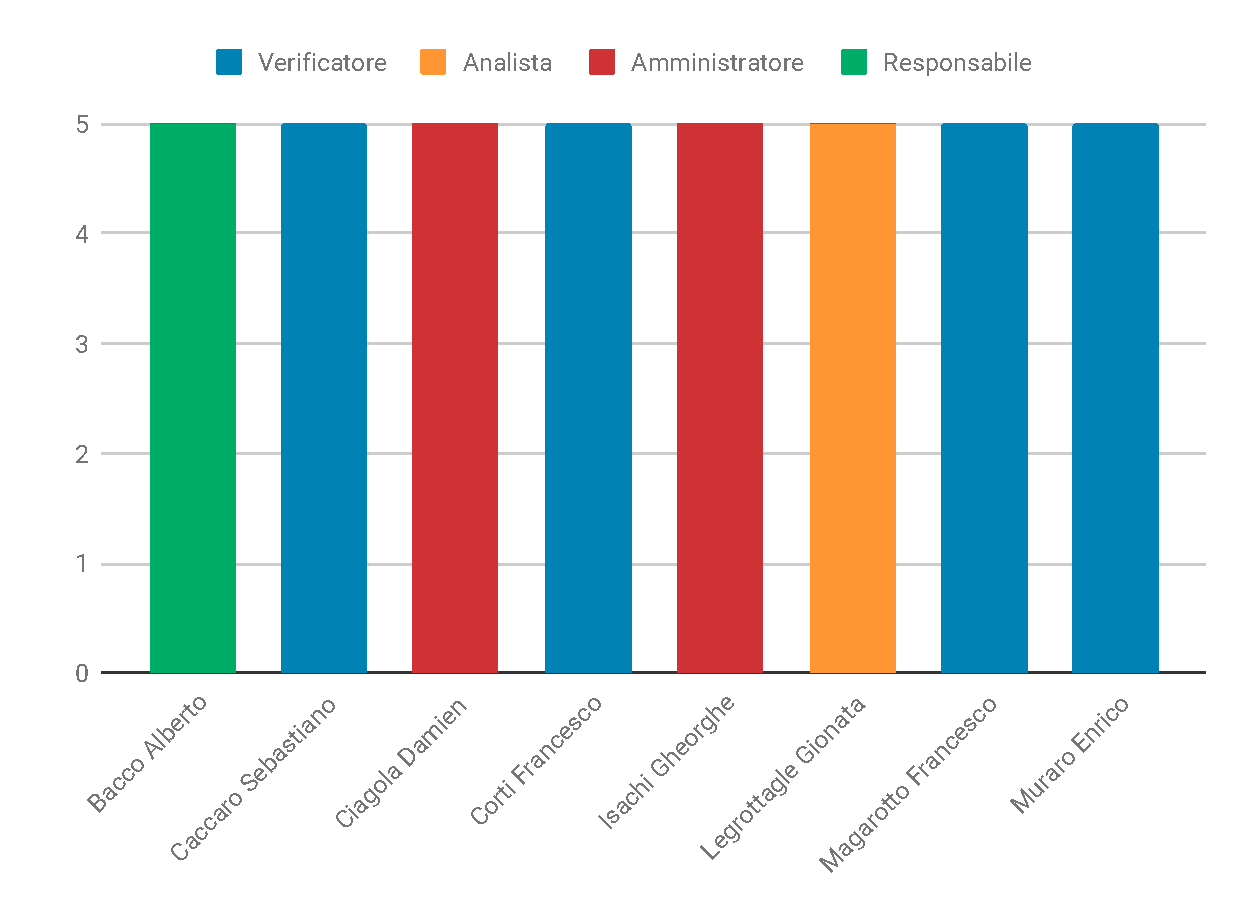
\includegraphics[width=1\linewidth]{Preventivo/grafici/CO1.pdf}
	\caption{Grafico della suddivisione oraria dei membri del gruppo nel periodo di Consolidamento}
\end{figure}

\subsubsection{Prospetto Economico}
Nella seguente tabella sono riportate le ore e i costi preventivati per ogni ruolo durante la fase di Consolidamento.


\begin{table}[H]	
	\begin{center}
	    \begin{tabular}{C{4cm}C{1cm}C{3,5cm}}
			\rowcolor{greySWEight}
			\textcolor{white}{\textbf{Ruolo}} & \textcolor{white}{\textbf{Ore}} & \textcolor{white}{\textbf{Costo}}
			\\ \hline
			Responsabile & 5 & \euro \space 150,00 \\
			Amministratore & 10 & \euro \space 200,00 \\
			Analista & 5 & \euro \space 125,00 \\
			Progettista &  & \\
			Programmatore &  &  \\
			Verificatore & 20 & \euro \space 300,00 \\
			\textbf{Totale} & \textbf{40} & \euro \space \textbf{775,00} \\
		\end{tabular}
	    \caption{Tabella della suddivisione oraria dei ruoli nel periodo di Consolidamento} \label{tab:tabellaRuoliConsolidamento} 
	\end{center}
\end{table}


Si può avere una più chiara rappresentazione della distribuzione oraria dei ruoli nel seguente grafico.

\begin{figure}[H]
	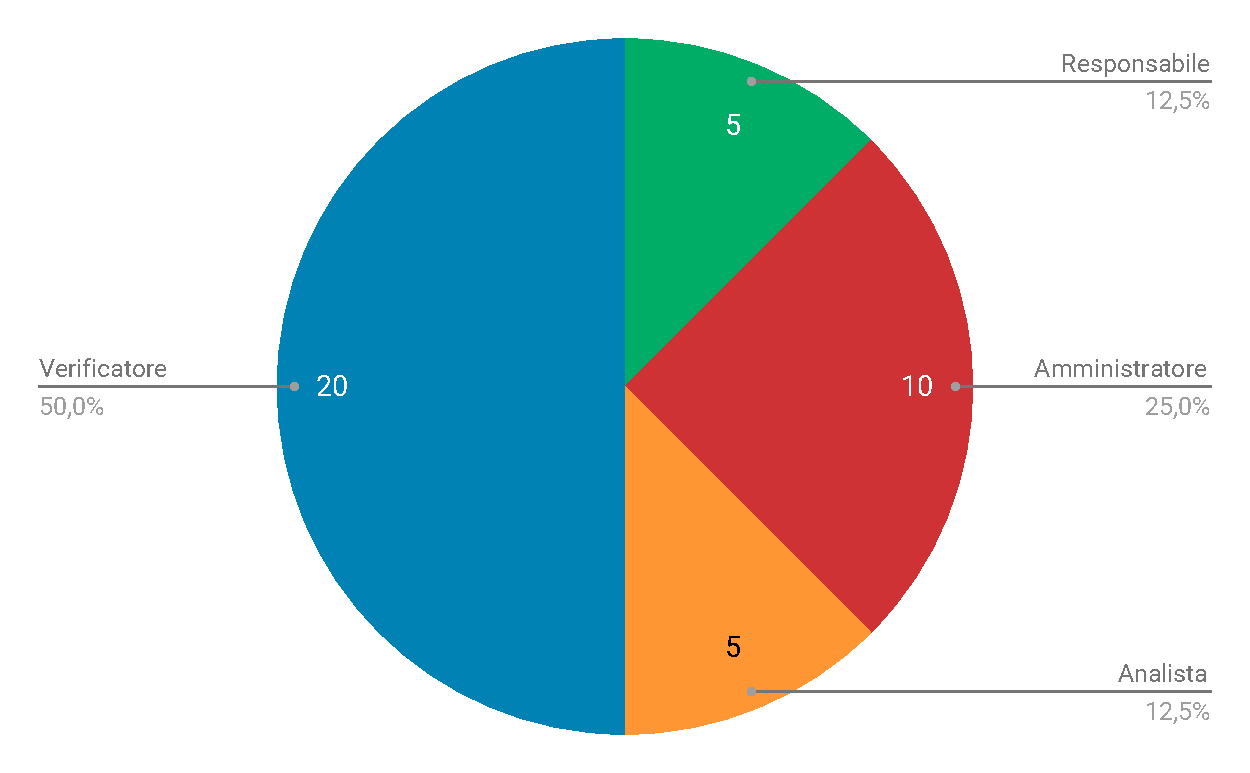
\includegraphics[width=1\linewidth]{Preventivo/grafici/CO2.pdf}
	\caption{Grafico della suddivisione oraria dei ruoli nel periodo di Consolidamento}
\end{figure}


	\newpage
	\subsection{Progettazione Architetturale}
	    \subsubsection{Prospetto Orario}
Di seguito è riportata la suddivisione oraria dei ruoli nel periodo di Progettazione Architetturale.




\begin{table}[H]	
	\begin{center}
	    \begin{tabular}{cccccccc}
			\rowcolor{greySWEight}
			\textcolor{white}{\textbf{Nome}} & \textcolor{white}{\textbf{Re}} & \textcolor{white}{\textbf{Am}} & \textcolor{white}{\textbf{An}} & \textcolor{white}{\textbf{Pj}} & \textcolor{white}{\textbf{Pr}} & \textcolor{white}{\textbf{Ve}} & \textcolor{white}{\textbf{Totale}}
			\\
			Bacco Alberto & 5 & & 7 & 5 & & 12 & 29 \\
			Caccaro Sebastiano & & & & 12 & & 17 & 29 \\
			Ciagola Damien & & & & 12 & & 17 & 29 \\
			Corti Francesco & & 5 & & 15 & & 9 & 29 \\
			Isachi Gheorghe & & & & 14 & & 15 & 29 \\
			Legrottagle Gionata & & & & 27 & & 2 & 29 \\
			Magarotto Francesco & 5 & & & 24 & & & 29 \\
			Muraro Enrico & & 5 & & 24 & & & 29 \\
			\end{tabular}
	    \caption{Tabella della suddivisione oraria dei membri del gruppo nel periodo di Progettazione Architetturale} \label{tab:tabellaPersoneProgettazione Architetturale} 
	\end{center}
\end{table}

La tabella della suddivisione oraria è rappresentata nel seguente grafico.
\begin{figure}[H]
	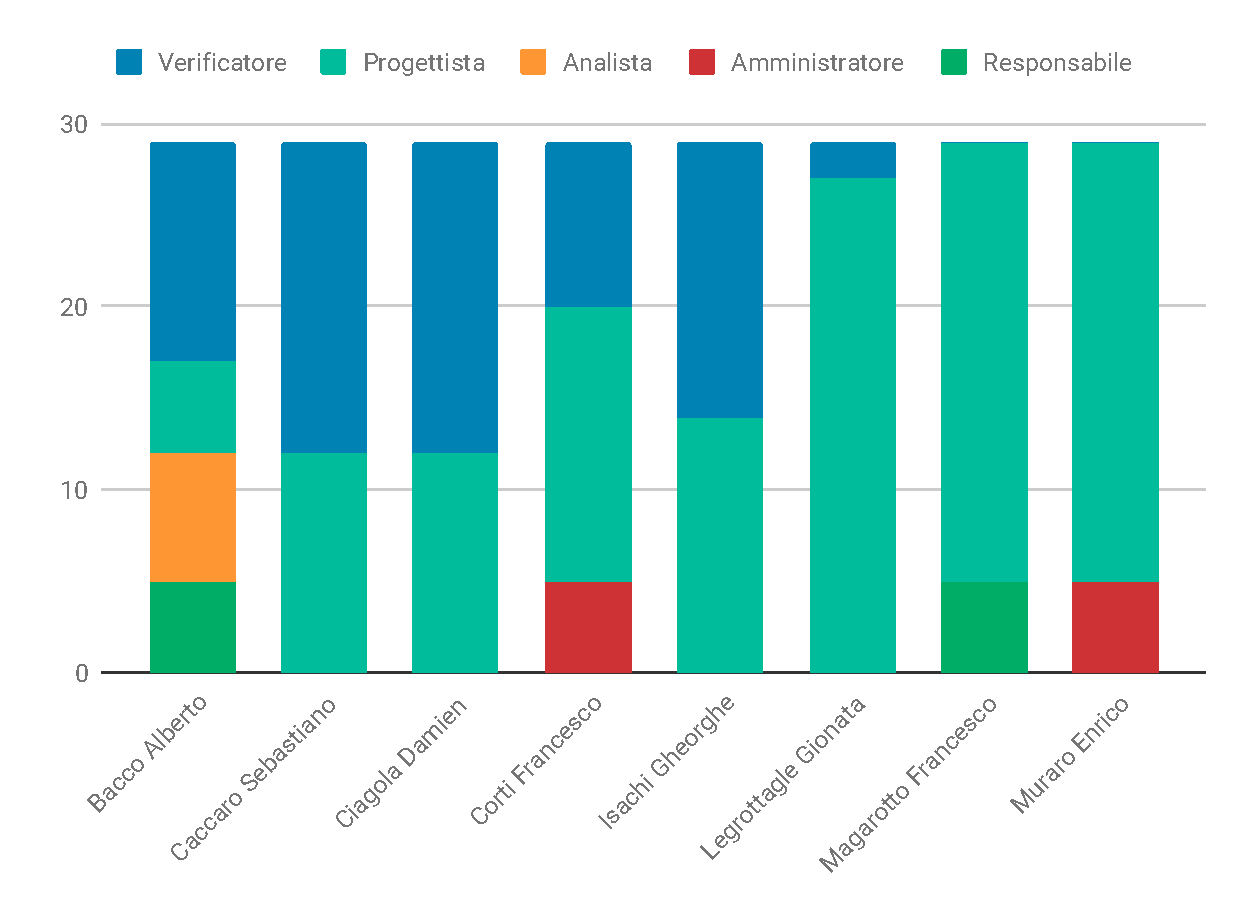
\includegraphics[width=1\linewidth]{Preventivo/grafici/PA1.pdf}
	\caption{Grafico della suddivisione oraria dei membri del gruppo nel periodo di Progettazione Architetturale}
\end{figure}

\subsubsection{Prospetto Economico}
Nella seguente tabella sono riportate le ore e i costi preventivati per ogni ruolo durante la fase di Progettazione Architetturale.


\begin{table}[H]	
	\begin{center}
	    \begin{tabular}{C{4cm}C{1cm}C{3,5cm}}
			\rowcolor{greySWEight}
			\textcolor{white}{\textbf{Ruolo}} & \textcolor{white}{\textbf{Ore}} & \textcolor{white}{\textbf{Costo}}
			\\
			Responsabile & 10 & \euro \space  300,00 \\
			Amministratore & 10 & \euro \space  200,00 \\
			Analista & 7 & \euro \space  175,00 \\
			Progettista & 133 & \euro \space  2.926,00 \\
			Programmatore &  & \euro \space  \\
			Verificatore & 72 & \euro \space  1.080,00 \\
			\textbf{Totale} & \textbf{232} & \euro \space  \textbf{4.681,00} \\
		\end{tabular}
	    \caption{Tabella della suddivisione oraria dei ruoli nel periodo di Progettazione Architetturale} \label{tab:tabellaRuoliProgettazione Architetturale} 
	\end{center}
\end{table}


Si può avere una più chiara rappresentazione della distribuzione oraria dei ruoli nel seguente grafico.

\begin{figure}[H]
	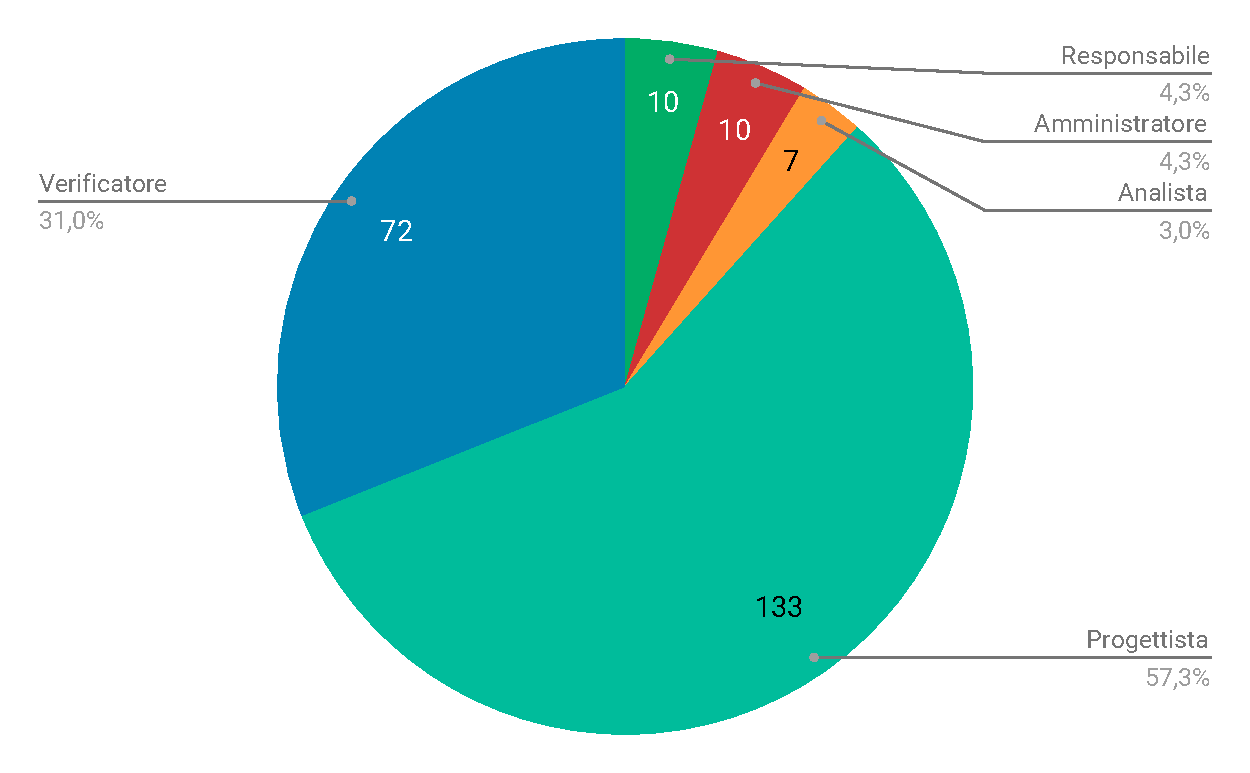
\includegraphics[width=1\linewidth]{Preventivo/grafici/PA2.pdf}
	\caption{Grafico della suddivisione oraria dei ruoli nel periodo di Progettazione Architetturale}
\end{figure}


	\newpage
	\subsection{Progettazione di Dettaglio e Codifica}
	    Il periodo di Progettazione di dettaglio e codifica inizia con la consegna della RP e termina con la consegna della RQ.\newline
Durante questo periodo, vengono svolte le seguenti attività:
\begin{itemize}
	\item \textbf{Incremento: }modifiche incrementali ai seguenti documenti, ove necessario:
	\begin{itemize}
		\item Analisi dei requisiti;
		\item Piano di progetto;
		\item Piano di qualifica;
		\item Glossario;
		\item Norme di progetto;
		\item Specifica Tecnica;
	\end{itemize}
	\item \textbf{Product Baseline: }sulla base della specifica tecnica viene redatto il documento di definizione di prodotto, nella quale sono contenute le scelte progettuali di dettaglio;
	\item \textbf{Codifica: }basandosi sulla definizione di prodotto, viene scritto il codice sorgente;
	\item \textbf{Manuale Utente: }redazione del manuale utente del prodotto. 
\end{itemize}


\begin{figure}[H]
	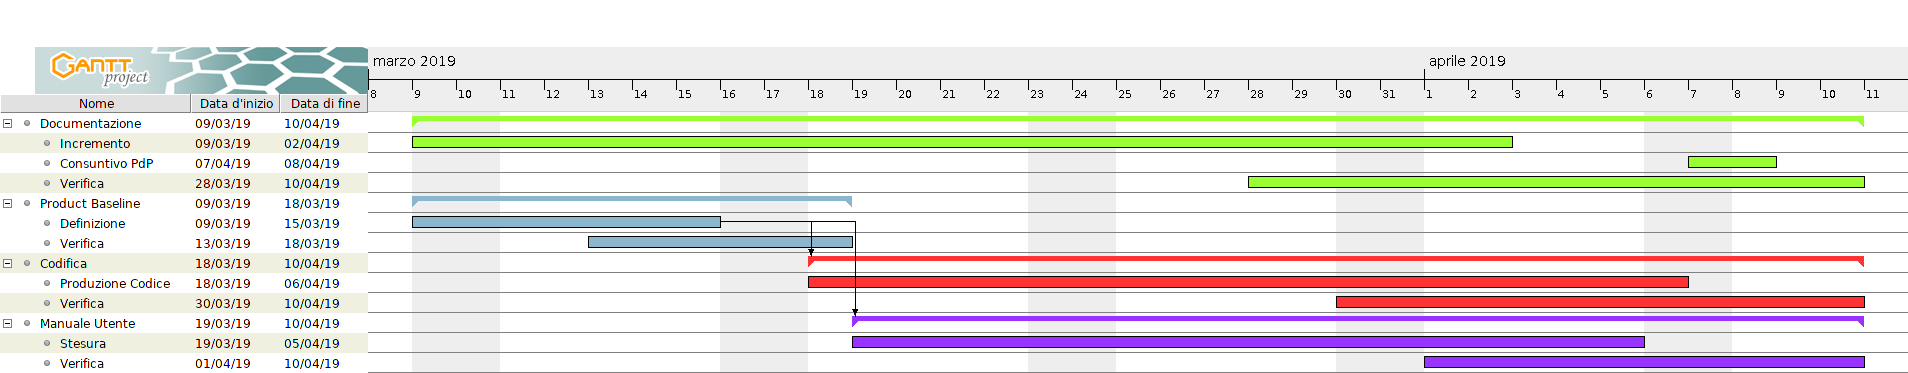
\includegraphics[width=1\linewidth]{Pianificazione/Progettazione_Dettaglio_Codififca.png}
	\caption{Diagramma di Gantt del periodo di Progettazione di dettaglio e codifica}
\end{figure}
	\newpage
	\subsection{Verifica e Validazione}
	\label{v&v}
	    Il periodo di verifica e validazione inizia con la consegna della RQ e termina con la consegna della RA.\newline
Durante questo periodo, sono svolte le seguenti attività:
\begin{itemize}
	\item \textbf{Incremento: }modifiche incrementali ai seguenti documenti, ove necessario:
	\begin{itemize}
		\item Analisi dei requisiti;
		\item Piano di progetto;
		\item Piano di qualifica;
		\item Glossario;
		\item Norme di progetto;
		\item Specifica Tecnica;
		\item Definizione di Prodotto;
		\item Manuale Utente;
	\end{itemize}
	\item \textbf{Validazione e collaudo: }il prodotto viene testato per accertarsi che soddisfi tutti i requisiti prestabiliti.
\end{itemize}


\begin{figure}[H]
	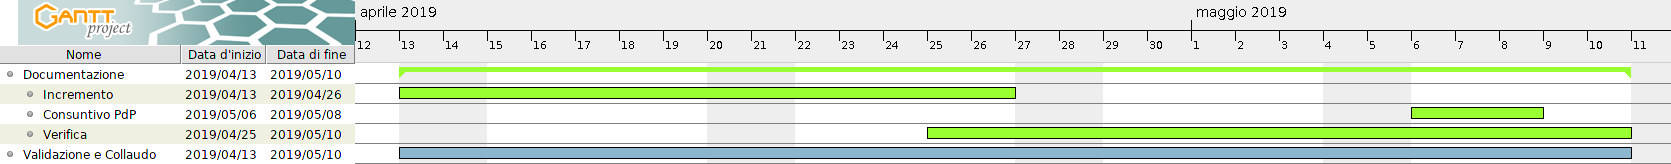
\includegraphics[width=1\linewidth]{Pianificazione/Verifica_Validazione.png}
	\caption{Diagramma di Gantt del periodo di verifica e validazione}
\end{figure}
	\newpage
	\subsection{Totale con Investimento}
	    \emph{IMPORTANTE: Questo preventivo, che include il periodo di investimento, ha scopo puramente informativo, e non è da intendersi come il preventivo finale da presentarsi alla proponente.}
\subsubsection{Prospetto Orario}
Di seguito è riportata la suddivisione oraria dei ruoli durante l'intera durata del progetto, \emph{compreso il periodo di investimento}.




\begin{table}[H]	
	\begin{center}
	    \begin{tabular}{cccccccc}
			\rowcolor{greySWEight}
			\textcolor{white}{\textbf{Nome}} & \textcolor{white}{\textbf{Re}} & \textcolor{white}{\textbf{Am}} & \textcolor{white}{\textbf{An}} & \textcolor{white}{\textbf{Pj}} & \textcolor{white}{\textbf{Pr}} & \textcolor{white}{\textbf{Ve}} & \textcolor{white}{\textbf{Totale}}
			\\
			Bacco Alberto & 10 & 5 & 17 & 27 & 10 & 59 & 128 \\
			Caccaro Sebastiano & 20 & 5 & 5 & 12 & 32 & 54 & 128 \\
			Ciagola Damien & 5 & 10 & 15 & 39 & 12 & 47 & 128 \\
			Corti Francesco & 5 & 10 & 20 & 15 & 22 & 56 & 128 \\
			Isachi Gheorghe & 5 & 5 & 5 & 36 & 20 & 57 & 128 \\
			Legrottagle Gionata & 5 & 15 & 5 & 49 & 20 & 34 & 128 \\
			Magarotto Francesco & 5 & 5 & 15 & 56 & 12 & 35 & 128 \\
			Muraro Enrico & 5 & 5 & 15 & 24 & 32 & 47 & 128 \\
			\end{tabular}
	    \caption{Tabella della suddivisione oraria dei membri del gruppo nell'intera durata del progetto} \label{tab:tabellaProgInt} 
	\end{center}
\end{table}

La tabella della suddivisione oraria è rappresentata nel seguente grafico.
\begin{figure}[H]
	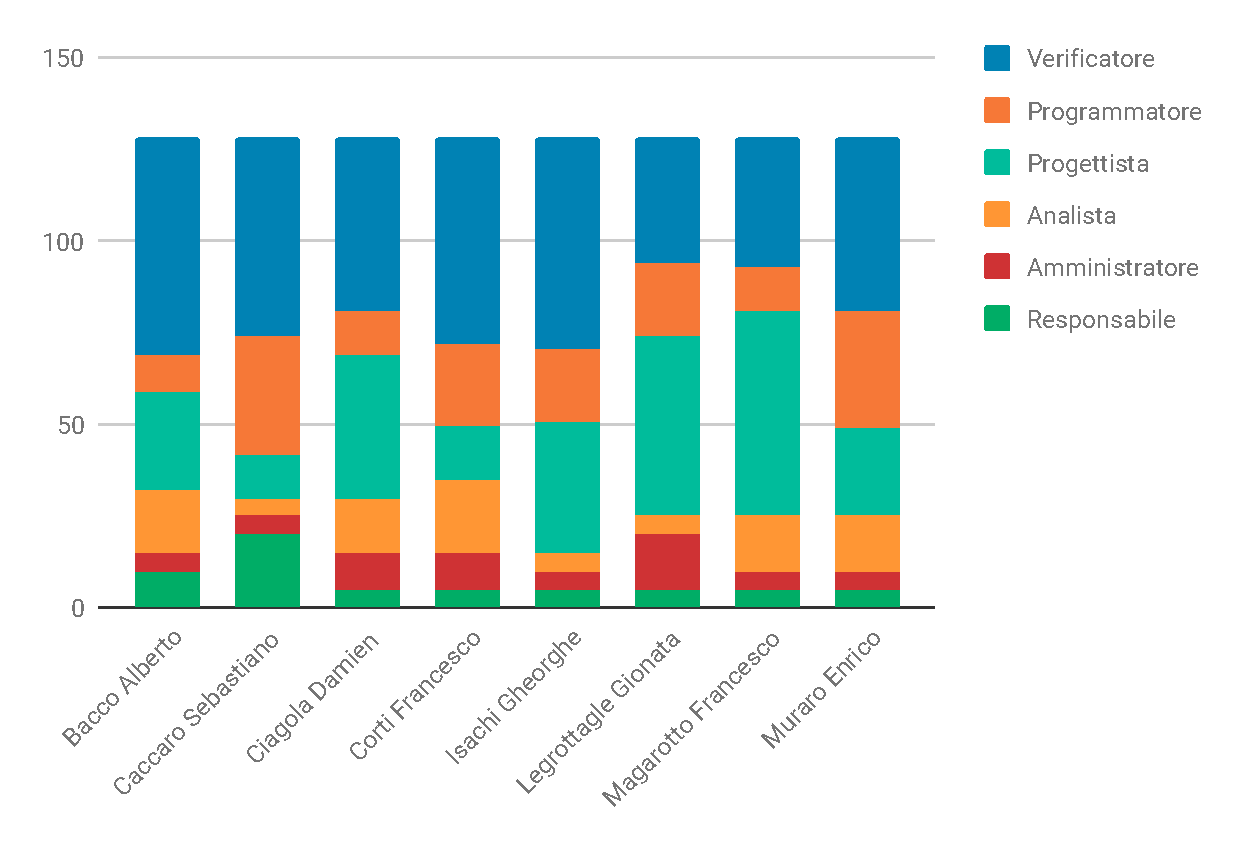
\includegraphics[width=1\linewidth]{Preventivo/grafici/TI1.pdf}
	\caption{Grafico della suddivisione oraria dei membri del gruppo nell'intera durata del progetto}
\end{figure}

\subsubsection{Prospetto Economico}
Nella seguente tabella sono riportate le ore e i costi preventivati per ogni ruolo durante tutta la durata del progetto, \emph{compreso il periodo di investimento}.


\begin{table}[H]	
	\begin{center}
	    \begin{tabular}{C{4cm}C{1cm}C{3,5cm}}
			\rowcolor{greySWEight}
			\textcolor{white}{\textbf{Ruolo}} & \textcolor{white}{\textbf{Ore}} & \textcolor{white}{\textbf{Costo}}
			\\
			Responsabile & 60 & \euro \space  1.800,00 \\
			Amministratore & 60 & \euro \space  1.200,00 \\
			Analista & 97 & \euro \space  2.425,00 \\
			Progettista & 258 & \euro \space  5.676,00 \\
			Programmatore & 160 & \euro \space  2.400,00 \\
			Verificatore & 389 & \euro \space  5.835,00 \\
			\textbf{Totale} & \textbf{1024} & \textbf{\euro \space  19.336,00} \\

		\end{tabular}
	    \caption{Tabella della suddivisione oraria dei ruoli nell'intera durata del progetto} \label{tab:tabellaRuoliProgInt} 
	\end{center}
\end{table}


Si può avere una più chiara rappresentazione della distribuzione oraria dei ruoli nel seguente grafico.

\begin{figure}[H]
	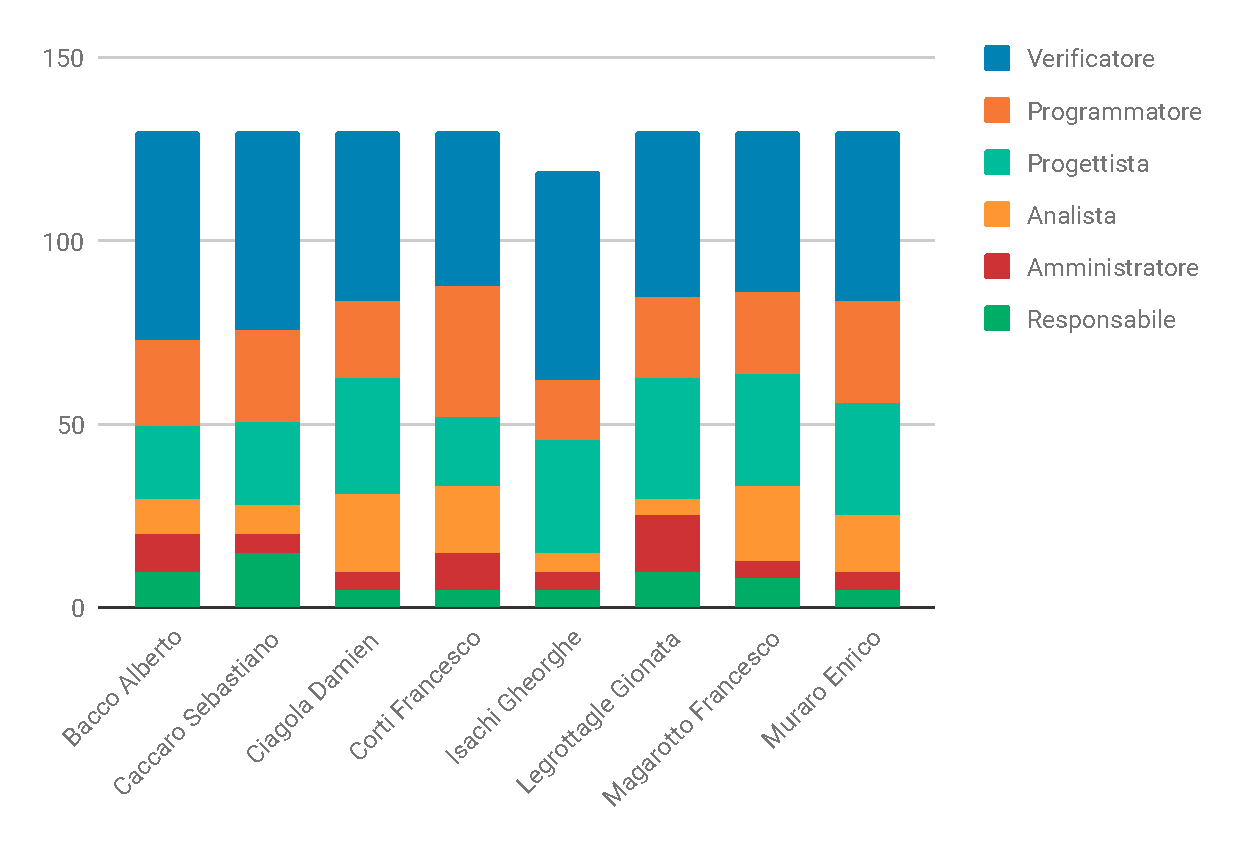
\includegraphics[width=1\linewidth]{Preventivo/grafici/TI2.pdf}
	\caption{Grafico della suddivisione oraria dei ruoli nell'intera durata del progetto}
\end{figure}


	\newpage
	\subsection{Totale Rendicontato}
	    \subsubsection{Prospetto Orario}
Di seguito è riportata la suddivisione oraria dei ruoli durante l'intera durata del periodo rendicontato del progetto.


\begin{table}[H]	
	\begin{center}
	    \begin{tabular}{cccccccc}
			\rowcolor{greySWEight}
			\textcolor{white}{\textbf{Nome}} & \textcolor{white}{\textbf{Re}} & \textcolor{white}{\textbf{Am}} & \textcolor{white}{\textbf{An}} & \textcolor{white}{\textbf{Pj}} & \textcolor{white}{\textbf{Pr}} & \textcolor{white}{\textbf{Ve}} & \textcolor{white}{\textbf{Totale}}
			\\			
			Bacco Alberto & 5 & 5 & 10 & 20 & 23 & 41 & 104 \\
			Caccaro Sebastiano & 0 & 5 & 4 & 26 & 24 & 45 & 104 \\
			Ciagola Damien & 5 & 0 & 2 & 27 & 30 & 40 & 104 \\
			Corti Francesco & 5 & 10 & 7 & 21 & 23 & 38 & 104 \\
			Isachi Gheorghe & 5 & 0 & 0 & 21 & 25 & 53 & 104 \\
			Legrottagle Gionata & 5 & 0 & 3 & 27 & 27 & 42 & 104 \\
			Magarotto Francesco & 8 & 5 & 0 & 33 & 33 & 25 & 104 \\
			Muraro Enrico & 5 & 5 & 3 & 30 & 24 & 37 & 104 \\

%			Bacco Alberto & 5 & 0 & 17 & 27 & 10 & 44 & 103 \\
%			Caccaro Sebastiano & 5 & 5 & 0 & 12 & 32 & 49 & 103 \\
%			Ciagola Damien & 5 & 5 & 0 & 39 & 12 & 42 & 103 \\
%			Corti Francesco & 5 & 10 & 5 & 15 & 22 & 46 & 103 \\
%			Isachi Gheorghe & 5 & 0 & 0 & 36 & 20 & 42 & 103 \\
%			Legrottagle Gionata & 0 & 0 & 0 & 49 & 20 & 34 & 103 \\
%			Magarotto Francesco & 5 & 5 & 0 & 56 & 12 & 25 & 103 \\
%			Muraro Enrico & 5 & 5 & 0 & 24 & 32 & 37 & 103 \\

			\end{tabular}
	    \caption{Tabella della suddivisione oraria dei membri del gruppo nel periodo rendicontato del progetto} \label{tab:tabellaPersoneTotale} 
	\end{center}
\end{table}

La tabella della suddivisione oraria è rappresentata nel seguente grafico.
\begin{figure}[H]
	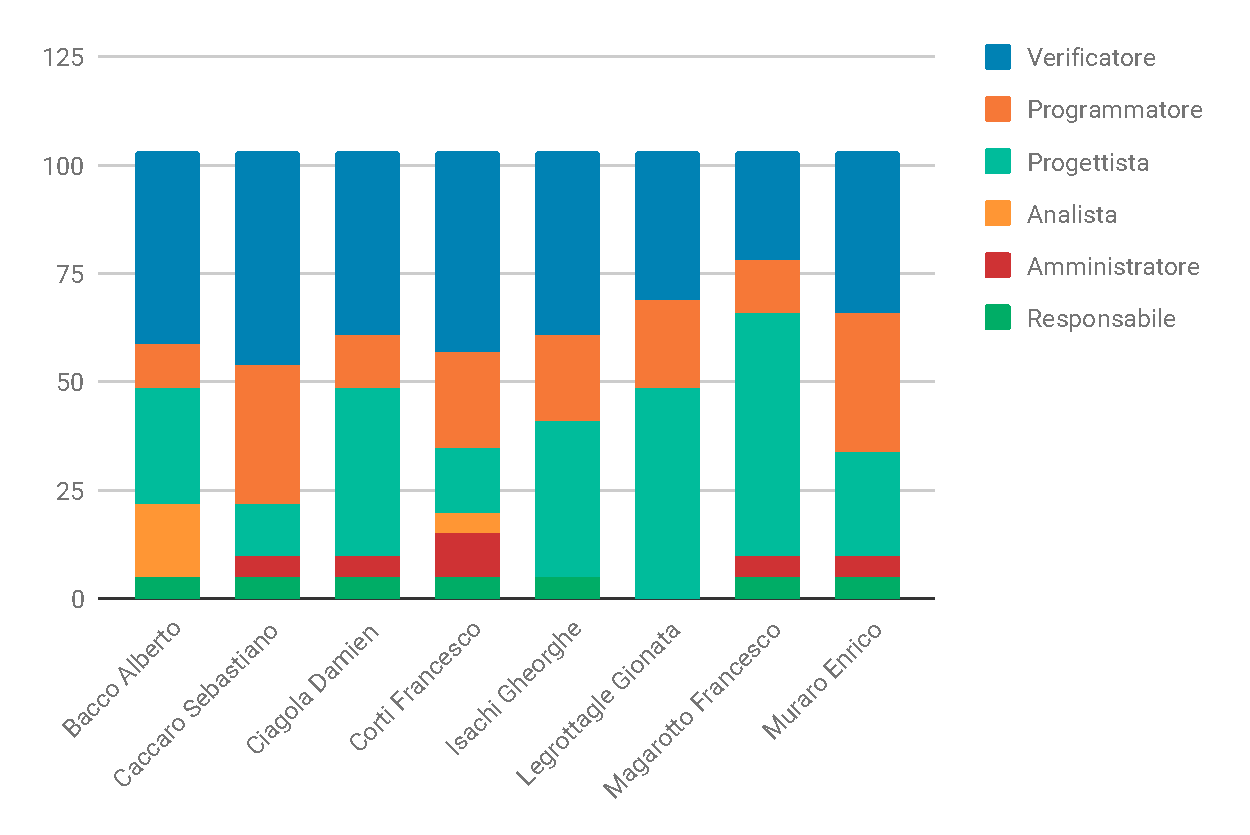
\includegraphics[width=1\linewidth]{Preventivo/grafici/TR1.pdf}
	\caption{Grafico della suddivisione oraria dei membri del gruppo nel periodo rendicontato del progetto}
\end{figure}

\subsubsection{Prospetto Economico}
Nella seguente tabella sono riportate le ore e i costi preventivati per ogni ruolo durante l'intera durata del periodo rendicontato del progetto.


\begin{table}[H]	
	\begin{center}
	    \begin{tabular}{C{4cm}C{1cm}C{3,5cm}}
			\rowcolor{greySWEight}
			\textcolor{white}{\textbf{Ruolo}} & \textcolor{white}{\textbf{Ore}} & \textcolor{white}{\textbf{Costo in €}}
			\\
			Responsabile & 35 & 1.050,00 \\
			Amministratore & 30 & 600,00 \\
			Analista & 22 & 550,00 \\
			Progettista & 258 & 5.676,00 \\
			Programmatore & 160 & 2.400,00 \\
			Verificatore & 319 & 4.785,00 \\
			\textbf{Totale} & \textbf{824} & \textbf{15.061,00} \\
		\end{tabular}
	    \caption{Tabella della suddivisione oraria dei ruoli nel periodo rendicontato del progetto} \label{tab:tabellaRuoliTotale} 
	\end{center}
\end{table}


Si può avere una più chiara rappresentazione della distribuzione oraria dei ruoli nel seguente grafico.

\begin{figure}[H]
	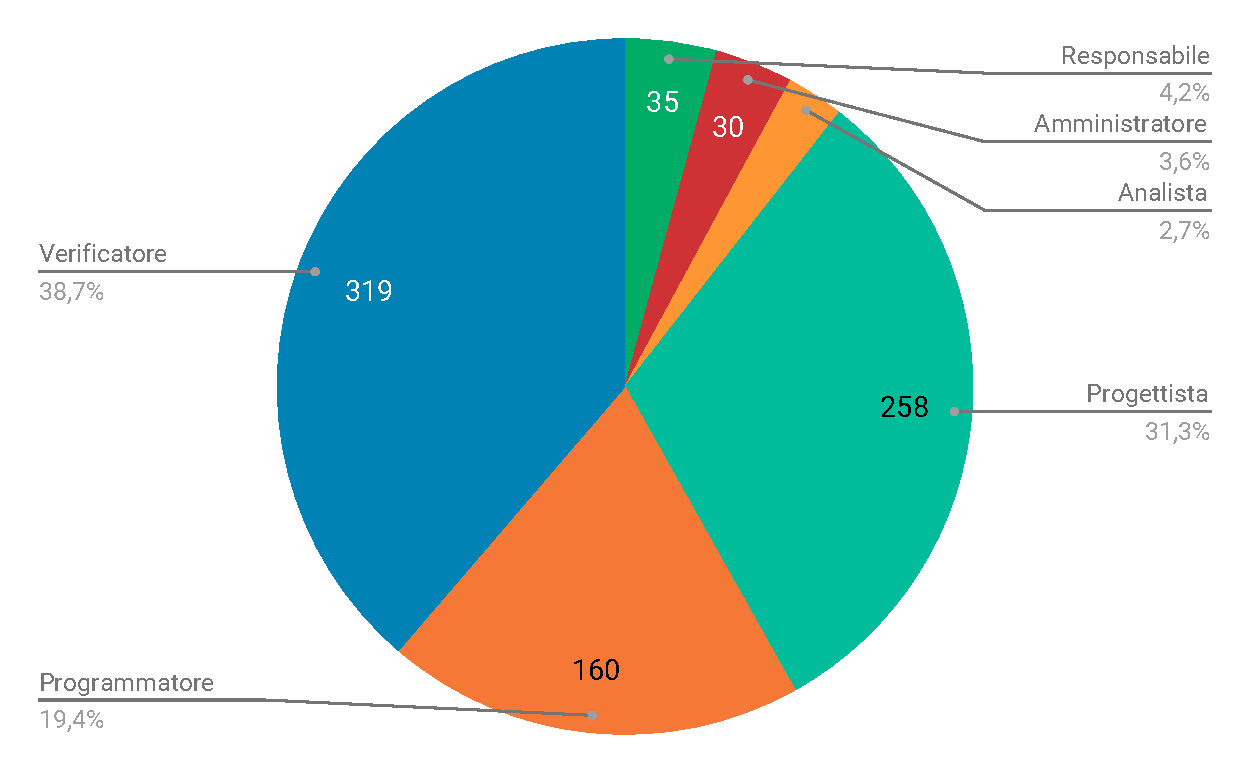
\includegraphics[width=1\linewidth]{Preventivo/grafici/TR2.pdf}
	\caption{Grafico della suddivisione oraria dei ruoli nel periodo rendicontato del progetto}
\end{figure}

	
\newpage
\section{Consuntivo e preventivo a finire}
	In questa sezione sono reperibili i consuntivi dei vari periodi e il preventivo a finire.\newline
Nelle tabelle dei consuntivi, la colonna \emph{Delta} indica la differenza tra quanto preventivato e quanto effettivamente consuntivato. Il Delta può essere:
\begin{itemize}
	\item \textbf{Positivo: }Si è lavorato o speso più di quanto preventivato;
	\item \textbf{Negativo: }Si è lavorato o speso meno di quanto preventivato;
	\item \textbf{Nullo: }Si è lavorato o speso tanto quanto si è preventivato.
\end{itemize}
	\subsection{Periodo di Analisi}
		Il periodo di Analisi è considerato un periodo di investimento, pertanto non verrà calcolato nel preventivo a finire. La sua presenza è a scopo puramente informativo.
		\subsubsection{Consuntivo}
			Nella seguente tabella è illustrato il consuntivo del periodo di Analisi.

\begin{table}[H]
\centering
\begin{tabular}{c|ccc|ccc}
\rowcolor{greySWEight}
\multicolumn{1}{c}{} & \multicolumn{3}{c}{\textcolor{white}{\textbf{Ore}}} & \multicolumn{3}{c}{\textcolor{white}{\textbf{Costo in Euro}}} \\
{\textbf{Ruolo}} & {\textbf{Preventivo}} & {\textbf{Consuntivo}} & {\textbf{Delta}} & {\textbf{Preventivo}} & {\textbf{Consuntivo}} & {\textbf{Delta}} \\
Responsabile & 20 & 24 & +4 &  600,00 &  720,00 & + 120,00 \\
Amministratore & 20 & 22 & +2 &  400,00 &  440,00 & + 40,00 \\
Analista & 70 & 74 & +4 &  1.750,00 &  1.850,00 & + 100,00 \\
Progettista & 0 & 0 & 0 &  0,00 &  0,00 &  0,00 \\
Programmatore & 0 & 0 & 0 &  0,00 &  0,00 &  0,00 \\
Verificatore & 50 & 46 & -4 &  750,00 &  690,00 & - 60,00 \\
\hline
\textbf{Totale} & \textbf{160} & \textbf{166} & \textbf{+6} &  \textbf{3.500,00} &  \textbf{3.700,00} & \textbf{+ 200,00} \\


\end{tabular}
\caption{Consuntivo del periodo di Analisi}
\end{table}

		\subsubsection{Osservazioni}
			Sono state necessarie più ore del previsto nei seguenti ruoli:
\begin{itemize}
	\item Responsabile;
	\item Amministratore;
	\item Analista.
\end{itemize}
Ciò è perlopiù da individuare in un'organizzazione iniziale non ottimale, che ha portato ad un rallentamento delle attività. Tale lacuna è stata in parte colmata nella parte finale del periodo, ed ulteriori provvedimenti verranno presi nel periodo di Consolidamento.
\newline
Sono state necessarie meno ore del previsto nei seguenti ruoli:
\begin{itemize}
	\item Verificatore.
\end{itemize}

	\newpage
	\subsection{Periodo di Consolidamento}
			Il periodo di Consolidamento è considerato un periodo di investimento, pertanto non verrà calcolato nel preventivo a finire. La sua presenza è a scopo prettamente informativo.
		\subsubsection{Consuntivo}
			\subsubsection{Prospetto Orario}
Di seguito è riportata la suddivisione oraria dei ruoli nel periodo di Consolidamento.




\begin{table}[H]	
	\begin{center}
	    \begin{tabular}{cccccccc}
	  		
			\rowcolor{greySWEight}
			\textcolor{white}{\textbf{Nome}} & \textcolor{white}{\textbf{Re}} & \textcolor{white}{\textbf{Am}} & \textcolor{white}{\textbf{An}} & \textcolor{white}{\textbf{Pj}} & \textcolor{white}{\textbf{Pr}} & \textcolor{white}{\textbf{Ve}} & \textcolor{white}{\textbf{Totale}}
			\\ \hline
			Bacco Alberto & 5 & & & & & & 5 \\
			Caccaro Sebastiano & & & & & & 5 & 5 \\
			Ciagola Damien & & 5 & & & & & 5 \\
			Corti Francesco & & & & & & 5 & 5 \\
			Isachi Gheorghe & & 5 & & & & & 5 \\
			Legrottagle Gionata & & & 5 & & & & 5 \\
			Magarotto Francesco & & & & & & 5 & 5 \\
			Muraro Enrico & & & & & & 5 & 5 \\

			\end{tabular}
	    \caption{Tabella della suddivisione oraria dei membri del gruppo nel periodo di Consolidamento} \label{tab:tabellaPersoneConsolidamento} 
	\end{center}
\end{table}

La tabella della suddivisione oraria è rappresentata nel seguente grafico.
\begin{figure}[H]
	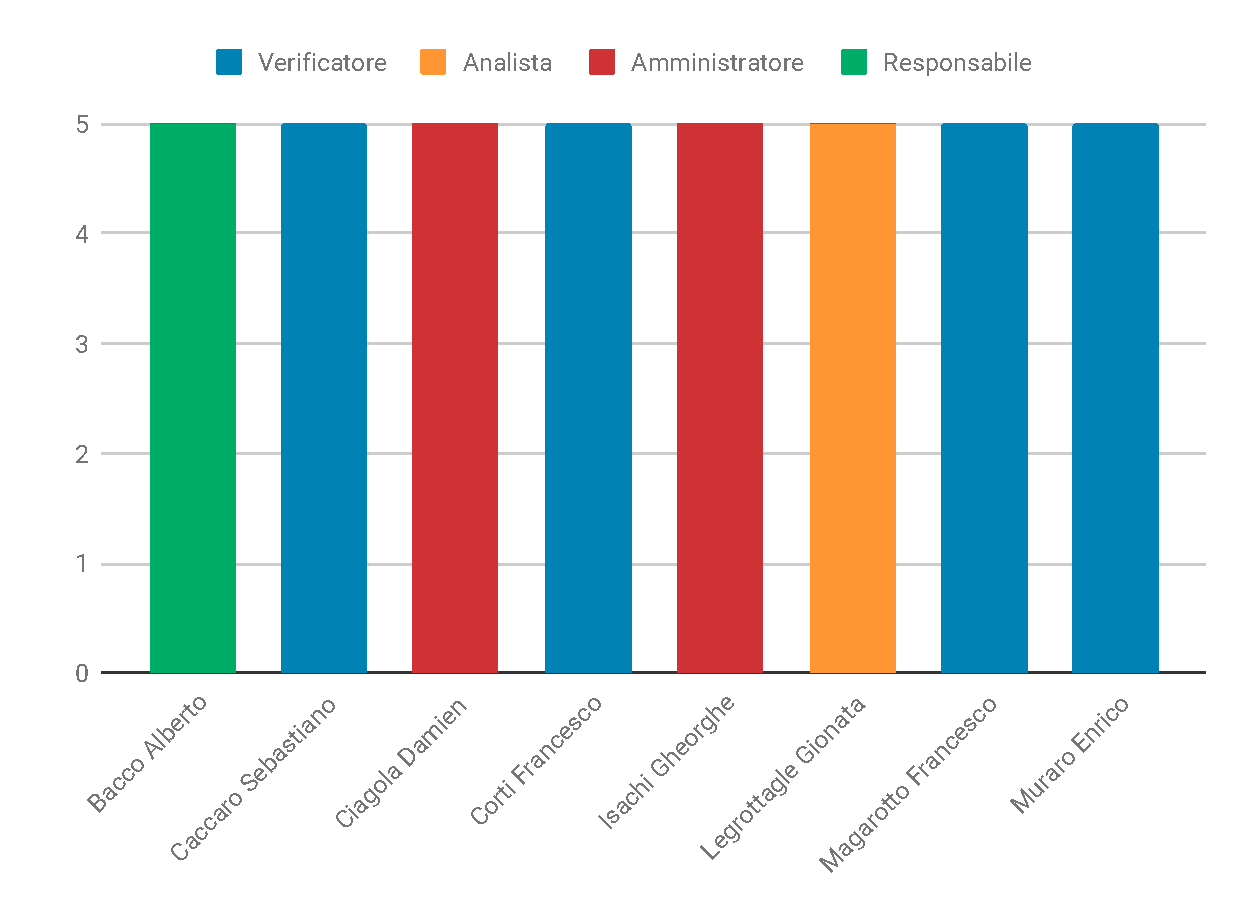
\includegraphics[width=1\linewidth]{Preventivo/grafici/CO1.pdf}
	\caption{Grafico della suddivisione oraria dei membri del gruppo nel periodo di Consolidamento}
\end{figure}

\subsubsection{Prospetto Economico}
Nella seguente tabella sono riportate le ore e i costi preventivati per ogni ruolo durante la fase di Consolidamento.


\begin{table}[H]	
	\begin{center}
	    \begin{tabular}{C{4cm}C{1cm}C{3,5cm}}
			\rowcolor{greySWEight}
			\textcolor{white}{\textbf{Ruolo}} & \textcolor{white}{\textbf{Ore}} & \textcolor{white}{\textbf{Costo}}
			\\ \hline
			Responsabile & 5 & \euro \space 150,00 \\
			Amministratore & 10 & \euro \space 200,00 \\
			Analista & 5 & \euro \space 125,00 \\
			Progettista &  & \\
			Programmatore &  &  \\
			Verificatore & 20 & \euro \space 300,00 \\
			\textbf{Totale} & \textbf{40} & \euro \space \textbf{775,00} \\
		\end{tabular}
	    \caption{Tabella della suddivisione oraria dei ruoli nel periodo di Consolidamento} \label{tab:tabellaRuoliConsolidamento} 
	\end{center}
\end{table}


Si può avere una più chiara rappresentazione della distribuzione oraria dei ruoli nel seguente grafico.

\begin{figure}[H]
	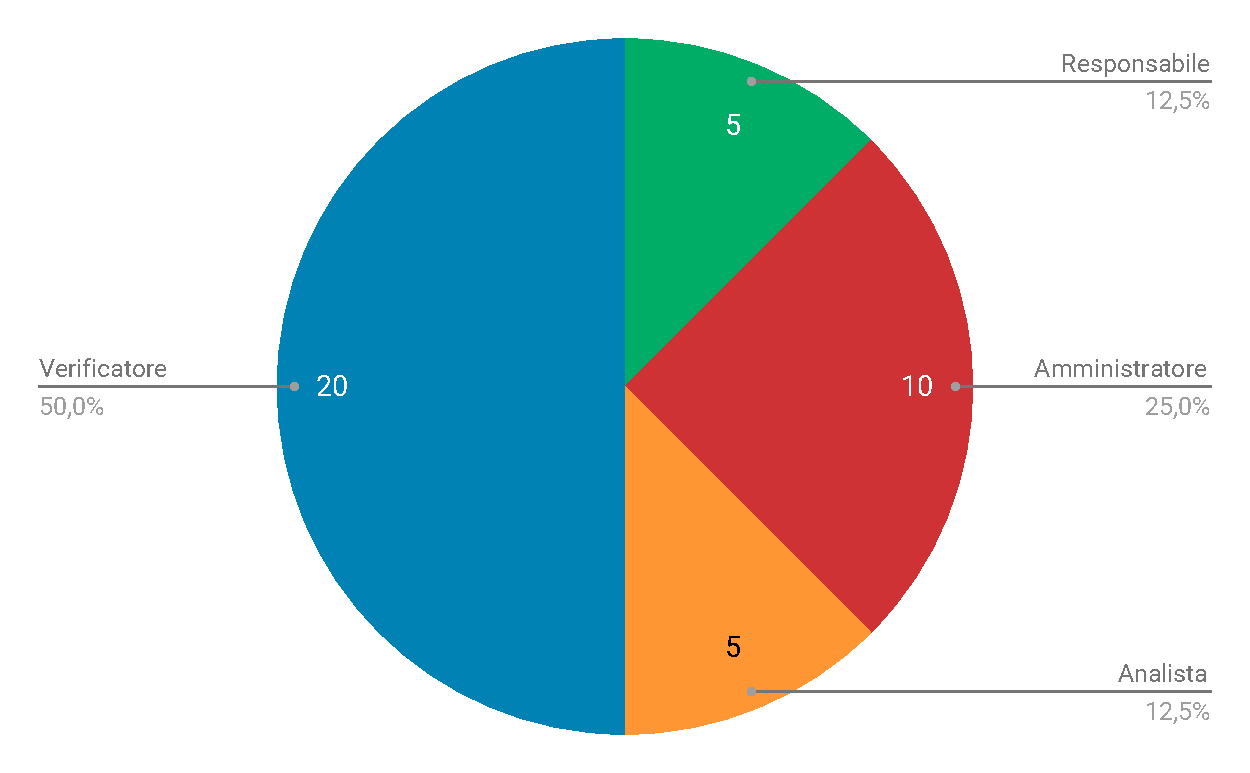
\includegraphics[width=1\linewidth]{Preventivo/grafici/CO2.pdf}
	\caption{Grafico della suddivisione oraria dei ruoli nel periodo di Consolidamento}
\end{figure}


		\subsubsection{Osservazioni}
			Sono state necessarie più ore per il ruolo di Analista rispetto a quanto era stato preventivato poiché sono state individuate alcune imprecisioni nei documenti presentati.
\newline
Sono state necessarie meno ore del previsto nei seguenti ruoli:
\begin{itemize}
	\item Verificatore;
\end{itemize}

	\newpage
	\subsection{Periodo di Progettazione Architetturale}
	Il periodo di Progettazione Architetturale è il primo periodo rendicontato del progetto. Esso consta nell'incremento della documentazione e nel delineare una Technology Baseline, ovvero una base solida sulle tecnologie e gli strumenti da utilizzare per realizzare il prodotto software. La concretizzazione di tali attività di formazione e scelta tecnologia si concretizza nella realizzazione di un Proof of Concept, un prototipo software funzionante che coinvolge le tecnologie scelte.
	\subsubsection{Consuntivo}
		Nella seguente tabella è illustrato il consuntivo del periodo di Progettazione Architetturale.


\begin{tabular}{c|ccc|ccc}
\rowcolor{greySWEight}
\multicolumn{1}{c}{} & \multicolumn{3}{c}{\textcolor{white}{\textbf{Ore}}} & \multicolumn{3}{c}{\textcolor{white}{\textbf{Costo in Euro}}} \\
{\textbf{Ruolo}} & {\textbf{Preventivo}} & {\textbf{Consuntivo}} & {\textbf{Delta}} & {\textbf{Preventivo}} & {\textbf{Consuntivo}} & {\textbf{Delta}} \\
Responsabile & 10 & 13 & 3 & 300,00 & 390,00 & 90,00 \\
Amministratore & 10 & 10 & 0 & 200,00 & 200,00 & 0,00 \\
Analista & 7 & 14 & 7 & 175,00 & 350,00 & 175,00 \\
Progettista & 133 & 80 & -53 & 2.926,00 & 1.760,00 & -1.166,00 \\
Programmatore & 0 & 49 & 49 & 0,00 & 735,00 & 735,00 \\
Verificatore & 72 & 74 & 2 & 1.080,00 & 1.110,00 & 30,00 \\
\hline
\textbf{Totale} & \textbf{232} & \textbf{240} & \textbf{+8} & \textbf{4.681,00} & \textbf{4.545,00} & \textbf{-136,00} \\
\end{tabular}
	\subsubsection{Osservazioni}
		La mancata comprensione delle attività richieste nel periodo di Progettazione Architetturale, in particolare riguardanti la Technology Baseline, ha portato ad alcuni cambiamenti rispetto al prospetto orario che era stato preventivato. In particolare, le ore destinate al ruolo di \textit{Progettista} non sono state svolte in toto, poiché durante questa fase non è richiesto progettare l'applicativo in tutte le sue parti, tale attività compete al periodo successivo alla di Progettazione in Dettaglio e Codifica. Infine, come si può notare dal consuntivo, sono state necessarie più ore di quelle preventivate per i seguenti ruoli:
\begin{itemize}
	\item \RdP{}: il \Res{} ha dovuto fare da mediatore all'interno dei componenti del gruppo soprattutto durante la fase di scelta degli strumenti tecnologici;
	\item \ana{}: per la correzione e l'incremento del documenti presentati in ingresso alla Revisione dei Requisiti e in seguito al colloquio avvenuto con la Proponente;
	\item \ver{}: per la verifica dei documenti che avevano necessità di un'ulteriore verifica conseguentemente al colloquio avvenuto con la Proponente;
	\item \progr{}: le ore per la realizzazione del PoC non erano state preventivate  in quanto non si erano comprese le richieste del Committente per la Revisione di Progettazione. 
\end{itemize} 
Questo ha portato ad un incremento delle ore preventivate per persona (29 ore) rendicontando un totale di 30 ore per componente.
Malgrado l'incremento orario, le ore da \textit{Progettista} non svolte ha portato un risparmio di \euro 136,00, tale valore non scende sotto la soglia minima richiesta dal Committente ma è da tenere sotto stretto controllo, in quanto sinonimo di una scarsa comprensione delle richieste avanzate dal Committente.

\paragraph{Attività future}\mbox{}\\
In considerazione degli errori commessi, si ritiene opportuno ripianificare le attività per i periodi futuri 
relativi alla Progettazione in Dettaglio e Codifica e alla Verifica e Validazione. 


%Le regole adottate per tale ridistribuzioni sono:
%\begin{itemize}
%	\item Il non superamento delle 105 ore individuali;
%	\item Il prezzo preventivato non può superare il valore stabilito alla Revisione dei Requisiti;
%	\item La quantità di investimento deve essere tenuta strettamente sotto controllo.
%\end{itemize}
%\newpage
%Per la Progettazione in Dettaglio e Codifica il prospetto orario che si propone è il seguente: 
%
%\begin{table}[H]	
%	\begin{center}
%	    \begin{tabular}{cccccccc}
%			\rowcolor{greySWEight}
%			\textcolor{white}{\textbf{Nome}} & \textcolor{white}{\textbf{Re}} & \textcolor{white}{\textbf{Am}} & \textcolor{white}{\textbf{An}} & \textcolor{white}{\textbf{Pj}} & \textcolor{white}{\textbf{Pr}} & \textcolor{white}{\textbf{Ve}} & \textcolor{white}{\textbf{Totale}}
%			\\ 
%			Bacco Alberto & & & 8 & 12 & 12 & 20 & 52 \\
%			Caccaro Sebastiano & & 5 & 2 & 17 & 13 & 15 & 52 \\
%			Ciagola Damien & & & & 20 & 12 & 20 & 52 \\
%			Corti Francesco & 5 & 5 & & 13 & 17 & 12 & 52 \\
%			Isachi Gheorghe & & & & 14 & 20 & 18 & 52 \\
%			Legrottagle Gionata & 5 & & & 17 & 10 & 20 & 52 \\
%			Magarotto Francesco & & & & 17 & 15 & 20 & 52 \\
%			Muraro Enrico & & & & 15 & 17 & 20 & 52 \\
%			\end{tabular}
%	    \caption{Tabella della suddivisione oraria proposta per i membri del gruppo nel periodo di Pianificazione di Dettaglio e Codifica} \label{tab:tabellaPropostaPersonePianificazione di dettaglio e codifica} 
%	\end{center}
%\end{table}
%\begin{figure}[H]
%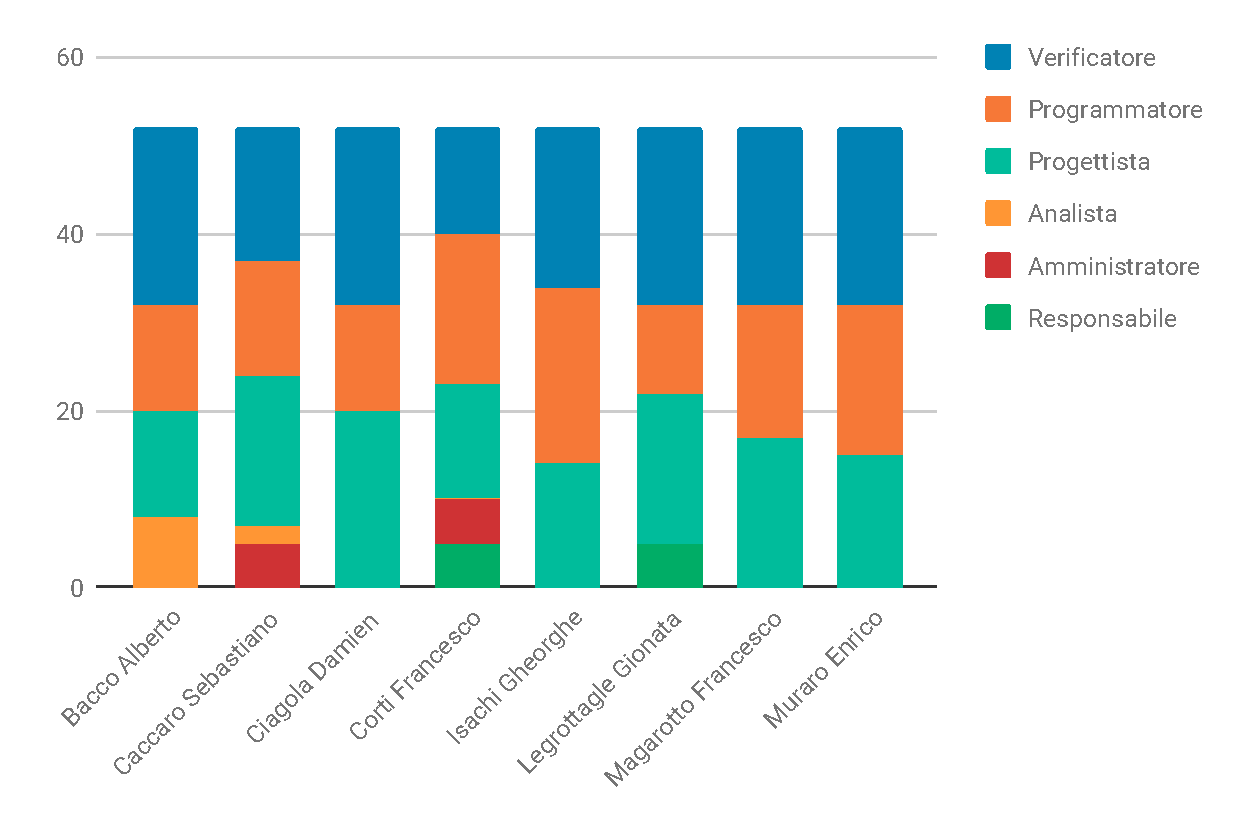
\includegraphics[width=1\linewidth]{Consuntivo/grafici/ConsPC1.pdf}
%\caption{Grafico ridistribuzione oraria per la Revisione di Qualifica proposto}
%\end{figure}
%
%Per quanto riguarda il periodo di Verifica e Validazione, il prospetto orario che viene proposto è il seguente:
%\begin{table}[H]	
%	\begin{center}
%	    \begin{tabular}{cccccccc}
%			\rowcolor{greySWEight}
%			\textcolor{white}{\textbf{Nome}} & \textcolor{white}{\textbf{Re}} & \textcolor{white}{\textbf{Am}} & \textcolor{white}{\textbf{An}} & \textcolor{white}{\textbf{Pj}} & \textcolor{white}{\textbf{Pr}} & \textcolor{white}{\textbf{Ve}} & \textcolor{white}{\textbf{Totale}}
%			\\
%			Bacco Alberto & & 5 & & & 5 & 12 & 22 \\
%			Caccaro Sebastiano & & & & & 5 & 17 & 22 \\
%			Ciagola Damien & 5 & & & & 12 & 5 & 22 \\
%			Corti Francesco & & & 5 & & & 17 & 22 \\
%			Isachi Gheorghe & 5 & & & & & 17 & 22 \\
%			Legrottagle Gionata & & & & & 10 & 12 & 22 \\
%			Magarotto Francesco & & 5 & & & 12 & 5 & 22 \\
%			Muraro Enrico & 5 & & & & & 17 & 22 \\
%			\end{tabular}
%	    \caption{Tabella della suddivisione oraria proposta per i membri del gruppo nel periodo di Verifica e Validazione} \label{tab:tabellaPropostaPersoneVerifica e validazione} 
%	\end{center}
%\end{table}
%\begin{figure}[H]
%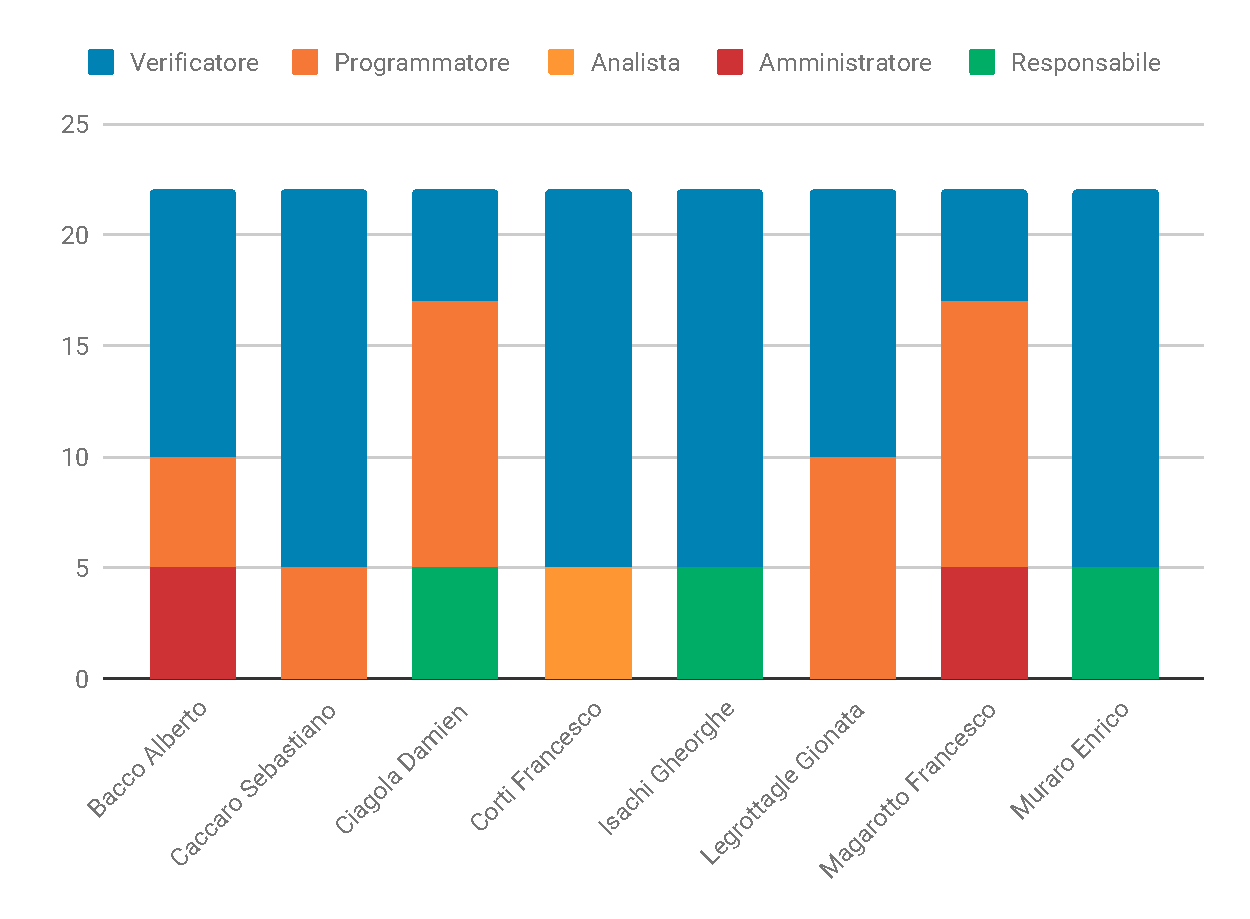
\includegraphics[width=1\linewidth]{Consuntivo/grafici/ConsVV1.pdf}
%\caption{Grafico ridistribuzione oraria per il periodo di Verifica e Validazione proposto}
%\end{figure}
Tali ridistribuzioni orarie devono lasciare invariato il costo preventivato senza modificare 
ore e ruoli dei componente del gruppo. Al contempo devono anche rispettare le seguenti direttive:
\begin{itemize}
	\item Uniformare la preparazione dei componenti. In quanto per il periodo di Progettazione in Dettaglio e Codifica per alcuni componenti non sono state preventivate ore di codifica;
	\item Permettere ad ogni componente del gruppo di svolgere almeno una volta ogni ruolo per un minimo di 5 ore durante tutto il progetto. 	
\end{itemize}
%In riferimento a quest'ultimo punto il grafico a seguire mostra le ore per componente durante il periodo rendicontato del progetto:
%\begin{figure}[H]
%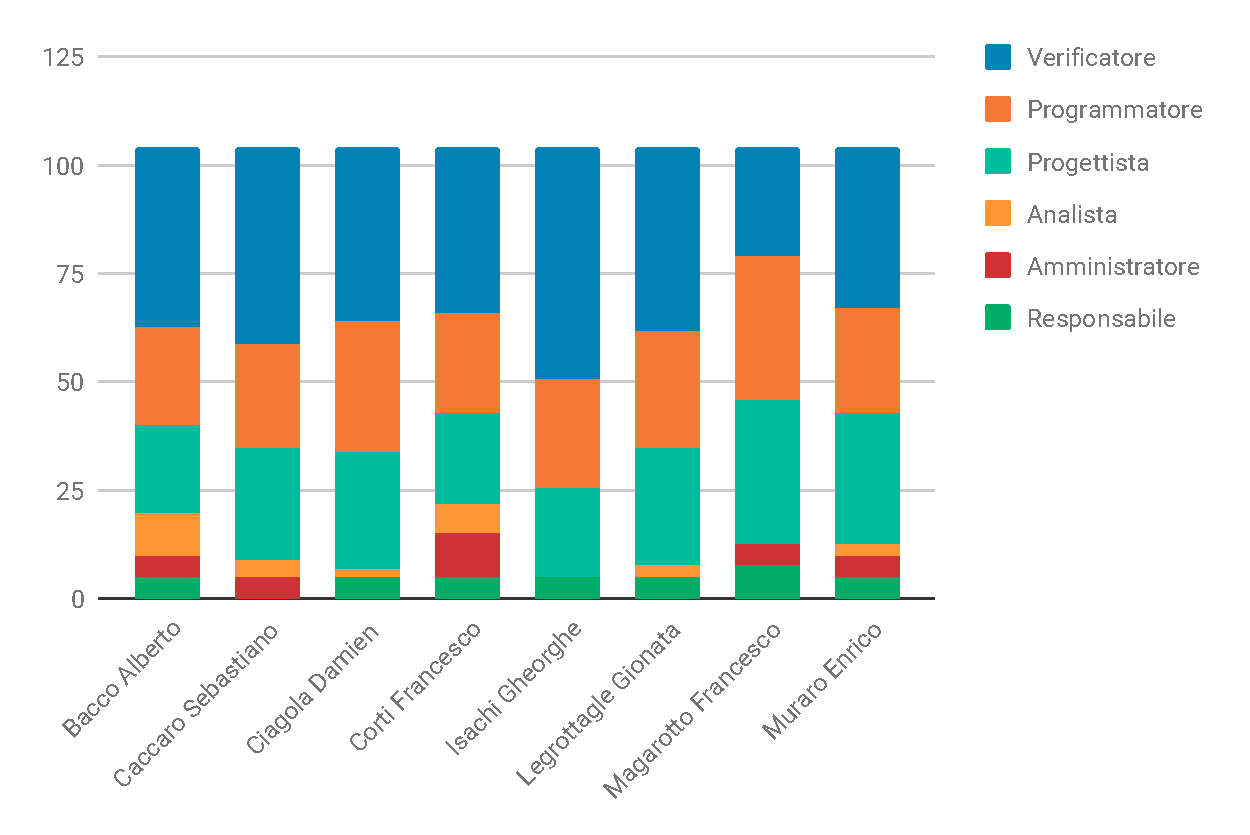
\includegraphics[width=1\linewidth]{Consuntivo/grafici/ConsTR1.pdf}
%\caption{Grafico ridistribuzione oraria reindicontata}
%\end{figure}

		
		
	\newpage
	\subsection{Periodo di Progettazione in dettaglio e Codifica}
	Il periodo di Progettazione Dettaglio e Codifica consta nell'incremento della documentazione e nel delineare l'architettura dell'applicativo, tramite un'accurata progettazione basata sulle tecnologie scelte alla Techonology Baseline. La concretizzazione delle attività di progettazione è documentata nell'\textit{Allegato tecnico v1.0.0}, presentato al docente Cardin tramite Hangouts. Inoltre, è necessario realizzare il \textit{Manuale Sviluppatore v1.0.0}, in lingua inglese, e il \textit{Manuale Utente v1.0.0} che descrive le funzionalità dell'applicativo.
	\subsubsection{Consuntivo}
		Nella seguente tabella è illustrato il consuntivo del periodo di Progettazione Dettaglio e Codifica.

\begin{tabular}{c|ccc|ccc}
\rowcolor{greySWEight}
\multicolumn{1}{c}{} & \multicolumn{3}{c}{\textcolor{white}{\textbf{Ore}}} & \multicolumn{3}{c}{\textcolor{white}{\textbf{Costo in Euro}}} \\
{\textbf{Ruolo}} & {\textbf{Preventivo}} & {\textbf{Consuntivo}} & {\textbf{Delta}} & {\textbf{Preventivo}} & {\textbf{Consuntivo}} & {\textbf{Delta}} \\
Responsabile & 10 & 10 & 0 & 300,00 & 300,00 & 0,00 \\
Amministratore & 10 & 10 & 0 & 200,00 & 200,00 & 0,00 \\
Analista & 10 & 13 & 3 & 250,00 & 325,00 & 75,00 \\
Progettista & 125 & 130 & 5 & 2.750,00 & 2.860,00 & 110,00 \\
Programmatore & 116 & 107 & -9 & 1.740,00 & 1.605,00 & -135,00 \\
Verificatore & 145 & 142 & -3 & 2.175,00 & 2.130,00 & -45,00 \\
\textbf{Totale} & \textbf{416} & \textbf{412} & \textbf{-4} & \textbf{7.415,00} & \textbf{7.420,00} & \textbf{5,00}\\

\end{tabular}
	\subsubsection{Osservazioni}
		Nella periodo di Progettazione in dettaglio e codifica l'impengo in ore dei singoli componenti del gruppo non è stato omogeo: la presenza di uno studente lavoratore a tempo pieno, impegato all'interno del settore dei trasporti, ha rallentato le attività di sviluppo del prodotto. In particolare, sono stati altri componenti a farsi carico di alcune ore non svolte. Tale difformità si manifesta anche nelle conoscenze dei singoli individui all'interno del gruppo: le tecnologie che vengono apprese soprattutto durante le attività di codifica e di progettazione, svolte durante tutta la settimana dagli studenti, portano alla creazione di un gap di conoscenze che è difficile sanare se non si segue constantemente il progetto. Il \RdP{} ha provveduto a contattare i singoli membri del gruppo che sono risultati poco attivi ed a informare il gruppo sull'andamento della situazione. Nonostante tali difficoltà, SWEight intende consegnare il progetto e participare alla \RA{} a Maggio, per permettere ai componenti in regola con gli esami di laurearsi nella sessione di Luglio. Il \RdP{} provvede ad attuare le seguenti strategie al fine di ridurre i rischi riscontrati e permettere la consegna del prodotto alla proponente:
\begin{itemize}
	\item Le attività di codifica verranno marginalmente affidate allo studente lavoratore al fine di fornigli conoscenza sulle tecnologie impiegate e ridurre il rischio di iterazione;
	\item Le attività di maggior importanza vengono iniziate il weekend al fine di permettere a coloro che lavorano di partecipare in maniera attiva;
	\item Ripianificazione periodo destinato alle attività di verifica e validazione.
\end{itemize}
Malgrado le problematiche sopra esposte i singoli componenti sono consapevoli che la situazione non può avere ampi margini di miglioramento e l'armonia all'interno del gruppo è buona.\\
\begin{figure}[H]
\centering
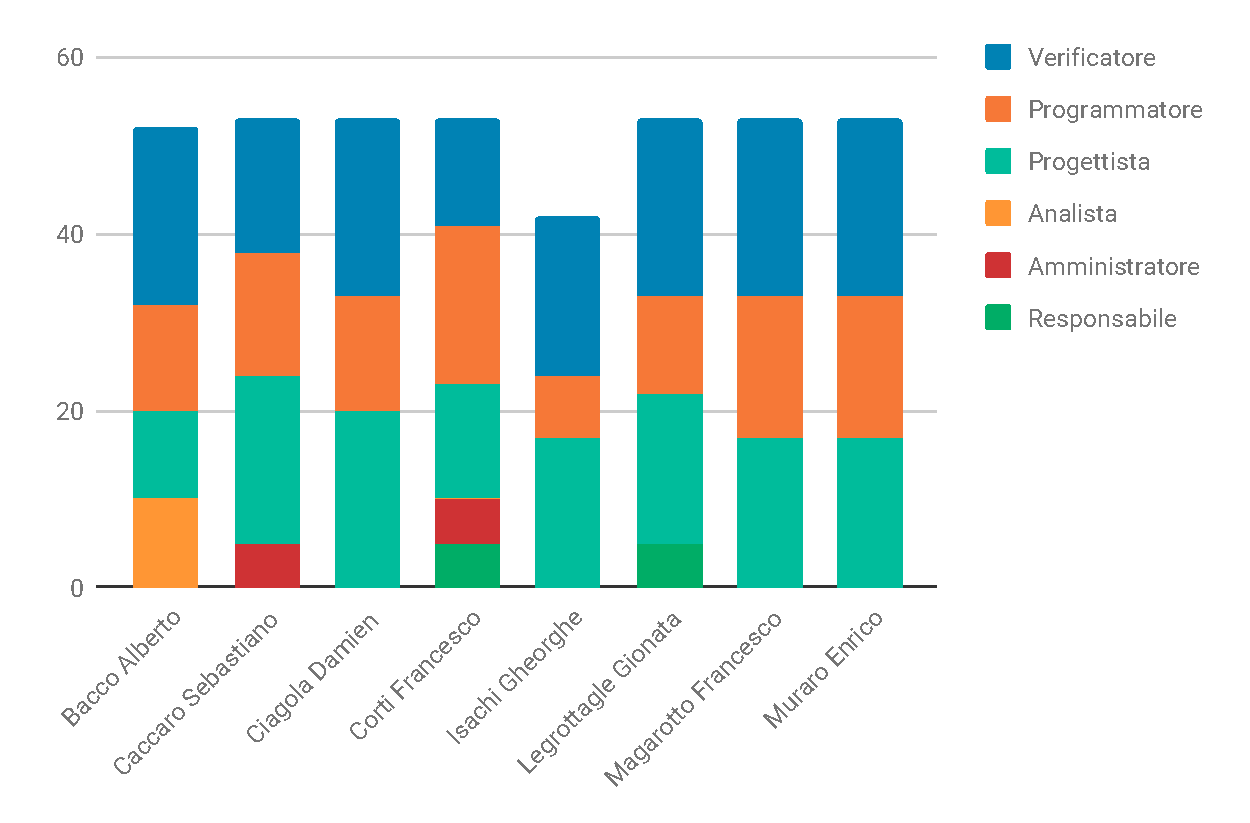
\includegraphics[scale=.8]{Consuntivo/grafici/ConsCod.pdf} 
\caption{Grafico orario per componente a fine periodo}
\end{figure}
\paragraph{Technology Baseline} \mbox{}\\
A seguito della \RP{} il gruppo ha provveduto a implementare una soluzione alternativa rispetto a quella proposta: il database Firestore è stato sostituito con MongoDB, alternativa open-source e pertanto priva di costi di licenza. Tale scelta è conseguente alla richiesta del docente Cardin di collegare il {database}\ped{G} alla backend al fine di ridurre l'accoppiamento. Lo studio di fattibilità di tale soluzione ha portato a complessità inaspettate, soprattutto nella stesura del codice Java, pertanto si è ritenuto provare ad implementare una nuova soluzione, dopo aver contattato e ottenuto l'approvazione da parte della proponente e dal docente Cardin. In relazione al fatto che entrambi i database sono documentali, pertanto la struttura delle collezioni è pressoché identica, e l'integrazione di Spring con MongoDB supportata dalla libreria Spring Data Mongo ha ridotto drasticamente la complessità del codice necessario. Pertanto, il cambio di tecnologia non ha portato a ritardi.
		\subsection{Preventivo a finire}
		Nella seguente tabella è riportato il consuntivo finale, che tiene conto del consuntivo di tutti i periodi. I periodi di investimento sono riportati solo a scopo informativo, e non sono inclusi nel totale rendicontato.

\begin{table}[H]
	\centering
	\begin{tabular}{ccc}
	\rowcolor{greySWEight}
	\textcolor{white}{\textbf{Periodo}} &
	\textcolor{white}{\textbf{Preventivo in Euro}} & 
	\textcolor{white}{\textbf{Costo in Euro}} \\
	Analisi & 3.500,00 & 3.700,00 \\
	Consolidamento & 775,00 & 795,00 \\
	\rowcolor{greySWEight}
	\multicolumn{3}{c}{ \textcolor{white}{\textbf{Rendicontato}} } \\
	Progettazione Architetturale & 4.681,00 & 4.545,00 \\
	Progettazione di Dettaglio e Codifica & 7.415,00 & 7.463,00 \\
	Verifica e Validazione & 2.957,00 & 2.978,00 \\
	\textbf{Totale} & \textbf{19.328,00} & \textbf{19.481,00} \\
	\textbf{Rendicontato} & \textbf{15.053,00} & \textbf{14.986,00} \\
	\multicolumn{2}{c}{\textbf{Totale preventivato in sede di \RR{}} } & \textbf{15.061,00} \\
	\end{tabular}
	\caption{Consuntivo finale}
\end{table}
\paragraph{Considerazioni}\mbox{}\\
Il costo finale si è mantenuto entro il valore preventivato, nonostante le e variazioni alle risorse orarie a causa delle criticità incontrate durante i vari periodi.
In conclusione, il costo totale rendicontato risulta di \textbf{13,263,00\euro{}} quindi inferiore al preventivo iniziale in sede di Revisione dei Requisiti, comportando un risparmio complessivo di \textbf{67\euro{}}

		
\appendix
\addcontentsline{toc}{part}{Appendici}

\newpage
\section{Riscontro Rischi}
	\label{app:riscontro}
	\subsection{Document goal}
The purpose of this document is to provide all the necessary information to extend, correct and improve Colletta.
There will be additional information regarding setting up the development environment to work in an environment that is as consistent as possible with that used
by the other members of group SWEight, but can be ignored if you only want to use part of the product.
This guide was written taking into account the Microsoft Windows and Linux operating systems. If other systems are used, compatibility issues may arise, even if it's unlikely. In this case refer to the git page. This document will grow as the product will be fully
developed.

\subsection{Product goal}
The purpose of the product is the creation of a collaborative data collection platform where users can prepare and/or perform small grammar exercises. 
The front-end of the system consists of a web application developed with React and Redux, while the back-end is a Spring Boot application written in Java, which will handle HTTP Requests sent from the front-end. 

\subsection{References}


\subsubsection{Installation references}

\begin{itemize}
\item \textbf{Git}: \url{https://git-scm.com/}
\item \textbf{Node.js}: \url{https://nodejs.org/en/}
\item \textbf{NPM}: \url{https://www.npmjs.com/}
\item \textbf{Oracle JDK}: \url{https://www.oracle.com/technetwork/java/javase/downloads/index.html}
\item \textbf{OpenJDK}: \url{https://openjdk.java.net/}
\item \textbf{Maven}: \url{https://maven.apache.org/}
\item \textbf{Lombok}: \url{https://projectlombok.org/}
\item \textbf{VSCode}: \url{https://code.visualstudio.com/} 

\end{itemize}

\subsubsection{Legal references}
\begin{itemize}
\item \textbf{MIT License}: \url{https://opensource.org/licenses/MIT}
\end{itemize}

%\subsubsection{Informative references}

	\subsection{Periodo di Analisi}
			Nella seguente tabella è descritto il riscontro dei rischi nel periodo di Analisi.

\renewcommand{\arraystretch}{1.5}
\def\tabularxcolumn#1{m{#1}}
\begin{tabularx}{\textwidth}{C{0.2\textwidth}XX}
\rowcolor{greySWEight}
    \textcolor{white}{\textbf{Codice\newline Nome}} &
    \textcolor{white}{\textbf{Descrizione}}&
    \textcolor{white}{\textbf{Soluzione}}%&
    %\textcolor{white}{\textbf{Correzione}}
    \endhead
    
%%%%%%%%%%%%%%%%%%%%%%%%%%%%%%%%%%%%%%%%%%%%%%%%%%%%%%%%%%%%%%%%%%%%%%
%%Nome
% \textbf{•}&
%
%%Descrizione
% &
%
%%Soluzione
% &
%
%%Correzione
% \\

%

%%%%%%%%%%%%%%%%%%%%%%%%%%%%%%%%%%%%%%%%%%%%%%%%%%%%%%%%%%%%%%%%%%%%%
%Nome
\textbf{A-001\newline Conflitti fra i membri del gruppo} &

%Descrizione
Alcune scelte divergenti, malintesi e fraintendimenti hanno creato dei micro-conflitti fra alcuni membri. &

%Soluzione
I membri in questione hanno contattato il responsabile. La natura non grave dei conflitti ha richiesto solo un po' di mediazione. Non sono stati presi altri provvedimenti.\\
\hline

%%%%%%%%%%%%%%%%%%%%%%%%%%%%%%%%%%%%%%%%%%%%%%%%%%%%%%%%%%%%%%%%%%%%%
%Nome
\textbf{A-002\newline Assenza prolungata di un membro del gruppo}&

%Descrizione
Alcuni membri hanno avuto l'impossibilità di lavorare per alcuni giorni per motivi familiari, di salute, o per mancanza di supporti informatici mentre in vacanza.&

%Soluzione
Quando possibile, il responsabile è stato avvertito con anticipo. Solo in un caso è stato richiesta una parziale redistribuzione del carico di lavoro.\\
\hline

%%%%%%%%%%%%%%%%%%%%%%%%%%%%%%%%%%%%%%%%%%%%%%%%%%%%%%%%%%%%%%%%%%%%%
%Nome
\textbf{B-001\newline Incompatibilità orari dei membri del gruppo}&

%Descrizione
Sopratutto nel periodo iniziale, è stata riscontrata una certa difficoltà nell'organizzazione delle riunioni.&

%Soluzione
Sono state organizzate riunioni tramite Google Hangouts.\\
\hline

%%%%%%%%%%%%%%%%%%%%%%%%%%%%%%%%%%%%%%%%%%%%%%%%%%%%%%%%%%%%%%%%%%%%%
%Nome
\textbf{M-001\newline Inesperienza tecnologica}&

%Descrizione
Alcuni membri hanno riscontrato difficoltà con l'uso di LaTex e Git/GitHub. &

%Soluzione
I membri più esperti con tali tecnologie hanno fornito risorse per l'apprendimento e aiuto ai componenti meno esperti.\\
\hline

%%%%%%%%%%%%%%%%%%%%%%%%%%%%%%%%%%%%%%%%%%%%%%%%%%%%%%%%%%%%%%%%%%%%%
%Nome
\textbf{A-003\newline Inesperienza organizzativa}&

%Descrizione
Sono state riscontrate alcune difficoltà nel tenere traccia dello svolgimento delle attività più complesse.&

%Soluzione
Sono stati necessari chiarimenti via Slack fra i membri del gruppo, e una maggiore gestione della coordinazione da parte del \Res . \\

Correzione &
\multicolumn{2}{L{\dimexpr\textwidth-4\tabcolsep-0.2\textwidth}}{
\'E necessaria una parziale rivisitazione della gestione delle attività, che verrà svolta nel periodo di consolidamento.
}\\
\hline
%

\rowcolor{white}
\caption{Riscontro dei rischi nel periodo di Analisi}
\end{tabularx}
	\subsection{Periodo di Progettazione Architetturale}
	Nella seguente tabella è descritto il riscontro dei rischi nel periodo di Progettazione Architetturale.

\renewcommand{\arraystretch}{1.5}
\def\tabularxcolumn#1{m{#1}}
\begin{tabularx}{\textwidth}{C{0.2\textwidth}XX}
\rowcolor{greySWEight}
    \textcolor{white}{\textbf{Nome}} &
    \textcolor{white}{\textbf{Descrizione}}&
    \textcolor{white}{\textbf{Soluzione}}%&
    %\textcolor{white}{\textbf{Correzione}}
    \endhead
    
\textbf{B-001\newline Incompatibilità orari dei membri del gruppo}&

%Descrizione
Alcuni componenti essendo studenti lavoratori full-time non hanno possibilità di controntarsi con gli altri membri durante la giornata.
&
%Soluzione
Sono state organizzate riunioni tramite Google Hangouts dopo l'orario lavorativo e tramite incontri fisici nei fine settimana.\\
\hline

%%%%%%%%%%%%%%%%%%%%%%%%%%%%%%%%%%%%%%%%%%%%%%%%%%%%%%%%%%%%%%%%%%%%%
%Nome
\textbf{M-001\newline Inesperienza tecnologica}&

%Descrizione
Alcuni membri hanno familiarità con le tecnologie scelte poiché utilizzate anche nel contesto lavorativo. Questo ha portato a creare un gap tra le conoscenze dei componenti del gruppo. &

%Soluzione
I membri più esperti con tali tecnologie hanno fornito risorse per l'apprendimento e hanno spiegato come realizzare il Proof of Concept e le tecnologie coivolte.\\
\hline

%%%%%%%%%%%%%%%%%%%%%%%%%%%%%%%%%%%%%%%%%%%
\textbf{M-003\newline Pianificazione fallacea}
   &
Nel periodo di Progettazione Architetturale non erano state preventivate ore per il ruolo di Programmatore per realizzare il PoC. 
   &  Il \RdP{} ha ripianificato le attività secondo le indicazioni pervenute dal docente. \\
   \hline
   %%%%%%%%%%%%%%%%%%%%%%%%%%
\textbf
   {A-005\newline Analisi dei requisiti incompleta}&
   La mancanza di un contatto, se non tramite email, con la proponente nel primo periodo ha portato, in alcuni punti dell'Analisi dei Requisiti, a creare casi d'uso incompleti o imprecisi. Inoltre, le lezioni tenute dal docente riguardo le aspettative del documento e il grado di precisione che ci si attend hanno chiarito i dubbi riguardanti l'attività di incremento per l'Analisi dei Requisiti. &
   Il \RdP{} ha provveduto a contattare la proponente che per un impegno lavorativo ha potuto indire una videochiamata solo una settimana prima della consegna ed predisposto le dovute attività di modifica.\\
\hline
\textbf
   {B-002\newline Divergenze per la Technology Baseline}&
   La scelta della base tecnologica ha creato alcune divergenze all'interno del gruppo sulle tecnologie da utilizzare &
   Il \RdP{} ha provveduto a trovare una soluzione che andasse bene a tutti i membri.\\
\hline
\rowcolor{white}
\caption{Riscontro dei rischi nel periodo di Progettazione Architetturale}
\end{tabularx}
	\subsection{Periodo di Progettazione in dettaglio e Codifica}
	Nella seguente tabella è illustrato il consuntivo del periodo di Progettazione Dettaglio e Codifica.

\begin{tabular}{c|ccc|ccc}
\rowcolor{greySWEight}
\multicolumn{1}{c}{} & \multicolumn{3}{c}{\textcolor{white}{\textbf{Ore}}} & \multicolumn{3}{c}{\textcolor{white}{\textbf{Costo in Euro}}} \\
{\textbf{Ruolo}} & {\textbf{Preventivo}} & {\textbf{Consuntivo}} & {\textbf{Delta}} & {\textbf{Preventivo}} & {\textbf{Consuntivo}} & {\textbf{Delta}} \\
Responsabile & 10 & 10 & 0 & 300,00 & 300,00 & 0,00 \\
Amministratore & 10 & 10 & 0 & 200,00 & 200,00 & 0,00 \\
Analista & 10 & 13 & 3 & 250,00 & 325,00 & 75,00 \\
Progettista & 125 & 130 & 5 & 2.750,00 & 2.860,00 & 110,00 \\
Programmatore & 116 & 107 & -9 & 1.740,00 & 1.605,00 & -135,00 \\
Verificatore & 145 & 142 & -3 & 2.175,00 & 2.130,00 & -45,00 \\
\textbf{Totale} & \textbf{416} & \textbf{412} & \textbf{-4} & \textbf{7.415,00} & \textbf{7.420,00} & \textbf{5,00}\\

\end{tabular}


\newpage
\section{Organigramma}
	\subsection{Redazione}
		\begin{table}[H]
	\centering
	\begin{tabular}{ccc}
	\rowcolor{greySWEight}
	    \textcolor{white}{\textbf{Nominativo}} &
	    \textcolor{white}{\textbf{Data}}&
	    \textcolor{white}{\textbf{Firma}}
    \\
    Sebastiano Caccaro &
    2019/01/06 &
    \firma{Caccaro}
    \\
    Gionata Legrottaglie &
    2019/01/06 &
    \firma{Legrottaglie}
    \\
    \hline
	\end{tabular}
	
	\caption{Redazione}
\end{table}
	\subsection{Approvazione}
		\begin{table}[H]
	\centering
	\begin{tabular}{ccc}
	\rowcolor{greySWEight}
	    \textcolor{white}{\textbf{Nominativo}} &
	    \textcolor{white}{\textbf{Data}}&
	    \textcolor{white}{\textbf{Firma}}
    \\
    Sebastiano Caccaro &
    2019-01-06 &
    \firma{Caccaro}
    \\
    Tullio Vardanega &
     &
    \firma{Vuoto}
    \\
    \hline
	\end{tabular}
	\caption{Approvazione}
\end{table}
	\subsection{Accettazione dei componenti}
		\begin{table}[H]
	\centering
	\begin{tabular}{ccc}
	\rowcolor{greySWEight}
	    \textcolor{white}{\textbf{Nominativo}} &
	    \textcolor{white}{\textbf{Data}}&
	    \textcolor{white}{\textbf{Firma}}
    \\
    Alberto Bacco &
    2019/01/07 &
    \firma{Bacco}
    \\
	Sebastiano Caccaro &
    2019/01/07 &
    \firma{Caccaro}
    \\
    Damien Ciagola &
    2019/01/07 &
    \firma{Ciagola}
    \\
    Corti Francesco &
    2019/01/07 &
    \firma{Corti}
    \\
    Gheorghe Isachi &
    2019/01/07 &
    \firma{Isachi}
    \\
    Gionata Legrottaglie &
    2019/01/07 &
    \firma{Legrottaglie}
    \\
    Francesco Magarotto &
    2019/01/07 &
    \firma{Magarotto}
    \\
    Enrico Muraro &
    2019/01/07 &
    \firma{Muraro}
    \\
    \hline
	\end{tabular}
	\caption{Accettazione dei componenti}
\end{table}	
	\subsection{Componenti}
		\begin{table}[H]
	\centering
	\begin{tabular}{ccc}
	\rowcolor{greySWEight}
	    \textcolor{white}{\textbf{Nominativo}} &
	    \textcolor{white}{\textbf{Matricola}}&
	    \textcolor{white}{\textbf{Email}}
    \\
    Alberto Bacco &
    1069129 &
    alberto.bacco.1@studenti.unipd.it 
    \\
    Sebastiano Caccaro &
    1142944 &
    sebastiano.caccaro@studenti.unipd.it 
    \\
    Damien Ciagola &
    1099107 &
    damien.ciagola@studenti.unipd.it 
    \\
    Corti Francesco &
    1142525 &
    francesco.corti@studenti.unipd.it 
    \\
    Gheorghe Isachi &
    1006498 &
    gheorghe.isachi@studenti.unipd.it 
    \\
    Gionata Legrottaglie &
    1102654 &
    gionata.legrottaglie@studenti.unipd.it 
    \\
    Francesco Magarotto &
    1143292 &
    francesco.magarotto@studenti.unipd.it 
    \\
    Enrico Muraro &
    1143775 &
    enrico.muraro.1@studenti.unipd.it 
    \\    
	\end{tabular}
	\caption{Componenti}
\end{table}

    

\end{document}